\documentclass[twocolumn,10pt,letterpaper]{article}

% Cargar configuración y paquetes
% Permite cortar las URL largas de la bibliografía también en los guiones
\PassOptionsToPackage{hyphens}{url}
\usepackage[utf8]{inputenc}
\usepackage[T1]{fontenc}
% english solo para partir bien las palabras del abstract; el idioma principal es spanish
\usepackage[english,spanish,es-tabla]{babel}
% El % sin espacio automático: el espacio se escribe a mano con \,
\spanishplainpercent
\decimalpoint

\usepackage{amsmath,amssymb,amsfonts}
\usepackage{graphicx}
\usepackage{geometry}
\usepackage{booktabs}
\usepackage{multirow}
\usepackage{array}
\usepackage{tabularx}
\usepackage{cite}
\usepackage{caption}
\usepackage{subcaption}
\usepackage{xcolor}
\usepackage{enumitem}
\usepackage{abstract}
\usepackage{titlesec}
\usepackage{verbatim} % Entorno comment que admite sangría antes de \end{comment}
\usepackage[colorlinks=true, linkcolor=blue, urlcolor=blue, citecolor=blue]{hyperref}

\graphicspath{{img/}}

% --- MÁRGENES ---
\geometry{
	letterpaper,
	top=2.0cm,
	bottom=2.0cm,
	left=1.8cm,
	right=1.8cm,
	columnsep=0.6cm
}

% --- FORMATO DE SECCIONES ---
\titleformat{\section}
{\normalfont\scshape\centering}
{\thesection.}
{0.5em}
{}

\renewcommand{\thesection}{\Roman{section}}

\titleformat{\subsection}
{\normalfont\itshape}
{\thesubsection.}
{0.5em}
{}

\renewcommand{\thesubsection}{\Alph{subsection}}

\titleformat{\subsubsection}[runin]
{\normalfont\itshape}
{}
{0em}
{}[.]

% --- CONFIGURACIÓN DEL RESUMEN ---
\renewcommand{\abstractname}{}
\setlength{\absleftindent}{0pt}
\setlength{\absrightindent}{0pt}

% Desactiva el título principal del resumen
\renewcommand{\abstractname}{}
\renewcommand{\absnamepos}{empty}
% Eliminar el título "Resumen" del entorno abstract por completo
\makeatletter
\renewenvironment{abstract}{%
	\small
	\par\noindent
}{%
	\par
}
\makeatother

% --- FIGURAS, TABLAS Y ALGORITMOS ---
\captionsetup{font=small, labelfont=bf, labelsep=period}
\captionsetup[sub]{font=footnotesize}
\setlist{nosep, leftmargin=*}

% Más espacio para flotantes en dos columnas
\renewcommand{\topfraction}{0.9}
\renewcommand{\bottomfraction}{0.8}
\renewcommand{\textfraction}{0.07}
\renewcommand{\floatpagefraction}{0.75}
\renewcommand{\dbltopfraction}{0.9}
\renewcommand{\dblfloatpagefraction}{0.75}
\setcounter{topnumber}{3}
\setcounter{dbltopnumber}{2}
\setcounter{totalnumber}{5}

\addto\captionsspanish{\renewcommand{\refname}{REFERENCIAS}}

% --- NOTACIÓN ---
% Arquitectura de la red: capas ocultas & capa de salida
\newcommand{\red}[2]{\mbox{#1}\,\&\,\mbox{#2}}
\newcommand{\onehot}{\textit{one-hot}}

% Paleta de los 18 estados de FLAME 3 (colores del simulador)
\definecolor{flame0}{HTML}{448CFD}\definecolor{flame1}{HTML}{17D9C7}\definecolor{flame2}{HTML}{2FF09A}
\definecolor{flame3}{HTML}{69FD65}\definecolor{flame4}{HTML}{A1FC3D}\definecolor{flame5}{HTML}{CDEB34}
\definecolor{flame6}{HTML}{EDCF39}\definecolor{flame7}{HTML}{FDA932}\definecolor{flame8}{HTML}{FA7A1F}
\definecolor{flame9}{HTML}{E84B0C}\definecolor{flame10}{HTML}{CB2B03}\definecolor{flame11}{HTML}{A01101}
\definecolor{flame12}{HTML}{000000}\definecolor{flame13}{HTML}{333333}\definecolor{flame14}{HTML}{666666}
\definecolor{flame15}{HTML}{999999}\definecolor{flame16}{HTML}{CCCCCC}\definecolor{flame17}{HTML}{FFFFFF}
\newcommand{\estadoflame}[2][black]{\fcolorbox{gray}{flame#2}{\makebox[0.9em]{\textcolor{#1}{\tiny #2}}}}
\newcommand{\leyendaflame}{%
	\par\smallskip
	{\scriptsize\setlength{\fboxsep}{0.8pt}%
	Temperatura: \estadoflame{0}\estadoflame{1}\estadoflame{2}\estadoflame{3}\estadoflame{4}\estadoflame{5}%
	\estadoflame{6}\estadoflame{7}\estadoflame{8}\estadoflame{9}\estadoflame[white]{10}\estadoflame[white]{11}%
	\quad Quemado: \estadoflame[white]{12}\estadoflame[white]{13}\estadoflame[white]{14}\estadoflame{15}%
	\estadoflame{16}\estadoflame{17}\par}}
% Versión en dos líneas para figuras de una columna
\newcommand{\leyendaflamecorta}{%
	\par\smallskip
	{\scriptsize\setlength{\fboxsep}{0.8pt}%
	Temperatura: \estadoflame{0}\estadoflame{1}\estadoflame{2}\estadoflame{3}\estadoflame{4}\estadoflame{5}%
	\estadoflame{6}\estadoflame{7}\estadoflame{8}\estadoflame{9}\estadoflame[white]{10}\estadoflame[white]{11}\\[1pt]
	Quemado: \estadoflame[white]{12}\estadoflame[white]{13}\estadoflame[white]{14}\estadoflame{15}%
	\estadoflame{16}\estadoflame{17}\par}}

% Paleta de los 7 estados de SEVIR
\definecolor{sevir0}{HTML}{F2F2F2}\definecolor{sevir1}{HTML}{9BE39B}\definecolor{sevir2}{HTML}{2E9E3A}
\definecolor{sevir3}{HTML}{F5D90A}\definecolor{sevir4}{HTML}{F28C1E}\definecolor{sevir5}{HTML}{D7191C}
\definecolor{sevir6}{HTML}{B10DC9}
\newcommand{\estadosevir}[2][black]{\fcolorbox{gray}{sevir#2}{\makebox[0.9em]{\textcolor{#1}{\tiny #2}}}}
\newcommand{\leyendasevir}{%
	\par\smallskip
	{\scriptsize\setlength{\fboxsep}{0.8pt}%
	Estado: \estadosevir{0}\estadosevir{1}\estadosevir[white]{2}\estadosevir{3}\estadosevir{4}%
	\estadosevir[white]{5}\estadosevir[white]{6}\par}}


\title{
	\textbf{\Large Simulación de sistemas complejos mediante \\ autómatas celulares neuronales}\\
}

\author{
	\normalsize Erick Jesse Angeles López, Genaro Juárez Martínez \\[0.2em]
	\small Escuela Superior de Cómputo I.P.N. México D.F. \\
	\small Tel. 57-29-6000 ext. 52000 y 52021. E-mail: \url{eangelesl1700@alumno.ipn.mx}
}

\date{}

\begin{document}

	\maketitle

	% Inclusión de secciones
	\begin{abstract}
	\noindent \textit{Resumen} --- \textbf{Los autómatas celulares se usan para simular sistemas complejos aplicando una regla local, conocida de antemano, a una condición inicial. En este trabajo se aborda el problema inverso: inferir la regla local a partir de la evolución observada de un sistema. Para ello, la función de transición del autómata se sustituye por un perceptrón multicapa entrenado con las transiciones de cada célula, lo que da lugar a un autómata celular neuronal bidimensional: discreto, determinista y síncrono, con estados escalares y sin canales ocultos. Se muestra que una regla determinista que reproduzca la evolución existe si la vecindad determina el siguiente estado. El modelo se evalúa en seis experimentos con un diseño cuasiexperimental. En tres sistemas con regla conocida (el juego de la vida, la pila de arena de Bak–Tang–Wiesenfeld y la hormiga de Langton con hasta 50 estados) el autómata reprodujo la evolución de las deficiones tradicionales sin errores y permitió definir una configuración recomendada: capas ocultas ReLU, salida lineal, codificación \textit{one-hot} y reducción por \textit{plateau}. En tres sistemas reales se obtuvo una regla que propaga el frente de fuego del conjunto FLAME~3 pero sin reproducir sus temperaturas por la falta de variables y de datos; y otra regla que mediante un valor de ruido incorporado al estado, reproduce el crecimiento de \textit{Physarum polycephalum}; el movimiento de tormentas de SEVIR, un sistema abierto, no pudo replicarse más allá de su desplazamiento hacia el este. Los resultados sugieren que la hipótesis se cumple en sistemas cerrados, en los que la vecindad contiene toda la información de la transición.}

	\begin{comment}
	\vspace{0.8em}
	\begin{otherlanguage}{english}
	\noindent \textit{Abstract} --- \textbf{Cellular automata are used to simulate complex systems by applying a local rule, defined beforehand, to an initial condition. This work addresses the inverse problem: inferring the local rule from the observed evolution of a system. To this end, the transition function of the automaton is replaced by a multilayer perceptron trained in a supervised way on the transitions of each cell, which yields a two-dimensional, discrete, deterministic and synchronous neural cellular automaton with scalar states and no hidden channels. It is shown that a deterministic rule that reproduces the evolution exists only if the neighborhood determines the next state, and the model is evaluated in six experiments with a quasi-experimental design. On three systems with a known rule (the Game of Life, the Bak–Tang–Wiesenfeld sandpile and Langton's ant with up to 50 states) the automaton reproduced its training evolution almost without errors and made it possible to define a recommended configuration: ReLU hidden layers, linear output, one-hot input encoding, plateau learning-rate reduction and a neighborhood that contains every relevant neighbor. On three real systems, a rule was obtained that spreads the fire front of the FLAME~3 dataset, although without reproducing its temperatures due to missing variables and scarce data, and, by adding a noise value to the state, a rule that reproduces the branching growth of \textit{Physarum polycephalum}; storm motion from SEVIR, an open system, could not be replicated beyond its eastward displacement. The results indicate that the hypothesis holds for closed systems, in which the neighborhood contains all the information of the transition.}
	\end{otherlanguage}

	\end{comment}

	\vspace{0.8em}
	\noindent \textit{Palabras clave} --- \textbf{Autómatas celulares, autómatas celulares neuronales, redes neuronales, sistemas complejos, simulación.}

	\begin{comment}
		
	\vspace{0.4em}
	\begin{otherlanguage}{english}
	\noindent \textit{Keywords} --- \textbf{Cellular automata, neural cellular automata, neural networks, complex systems, simulation.}
	\end{otherlanguage}
	
	\end{comment}
	
\end{abstract}

	\section{INTRODUCCIÓN}

Los autómatas celulares son una herramienta de simulación de sistemas complejos que permite estudiar fenómenos en los que muchas interacciones locales producen un comportamiento global que no puede deducirse de cada parte por separado. Desde los trabajos de von Neumann \cite{neumann1966_ca} y su popularización por Wolfram \cite{wolfram1982_ca}, los autómatas celulares se han consolidado como uno de los modelos más simples capaces de exhibir este tipo de dinámicas emergentes \cite{Hoekstra2010_cs_ca}. Formalmente, un autómata celular es una 4-tupla $(\mathcal{L}, \mathcal{S}, \mathcal{N}, \mathcal{R})$ \cite{weisstein2002_ca, ZenilMartinez2024} donde:

\begin{itemize}
	\item $\mathcal{L} \subseteq \mathbb{Z}^D$ es el espacio celular $D$-dimensional, en el que cada célula $\vec{i}$ ocupa una posición.
	\item $\mathcal{S} = \{s_0, s_1, \dots, s_{k-1}\}$ es un conjunto finito de $k$ estados; $\sigma_{\vec{i}}(t) \in \mathcal{S}$ es el estado de la célula $\vec{i}$ en el tiempo $t$.
	\item $\mathcal{N} = (\vec{v}_1, \dots, \vec{v}_m)$ es el conjunto de $m$ vectores de desplazamiento que definen la vecindad: los vecinos de $\vec{i}$ son las células $\vec{i} + \vec{v}_j$.
	\item $\mathcal{R} : \mathcal{S}^m \to \mathcal{S}$ es la regla local, que todas las células aplican de forma simultánea:
\end{itemize}
\begin{equation}
	\sigma_{\vec{i}}(t+1) = \mathcal{R}\left(\sigma_{\vec{i}+\vec{v}_1}(t), \dots, \sigma_{\vec{i}+\vec{v}_m}(t)\right).
	\label{eq:regla_local}
\end{equation}

El uso tradicional de los autómatas celulares define la regla $\mathcal{R}$ y se observa la evolución que produce a partir de una condición inicial. Sin embargo, para simular un sistema real es necesario conocer de antemano su regla, que en la mayoría de los fenómenos naturales se desconoce. Buscarla a mano tampoco es viable: el número de reglas posibles es $k^{k^m}$, por lo que con solo dos estados y la vecindad de Moore ($m = 9$) ya existen $2^{512}$ reglas, y el modelo de pila de arena que se estudia en este trabajo, con 17 estados y la vecindad de von Neumann, es una entre $17^{17^5}$ \cite{elYacoubi2021control}.

En este trabajo se plantea el problema inverso: dada la evolución observada $\{\sigma(t)\}_{t=0}^{T}$ de un sistema, encontrar una regla local que la reproduzca. Para ello, la regla $\mathcal{R}$ se sustituye por una red neuronal $F_\theta$ que se entrena con las transiciones observadas de cada célula, lo que da lugar a los autómatas celulares neuronales \cite{gilpin2019_nca, mordvintsev2020_nca}. Una vez entrenada, la red se aplica como cualquier otra regla local y permite extrapolar el comportamiento a nuevas condiciones iniciales. La pregunta no es si la red aprende, sino en qué condiciones la evolución observada contiene la información necesaria para inferir la regla.

\subsection{Trabajos relacionados}

Gilpin \cite{gilpin2019_nca} mostró que los autómatas celulares y las redes neuronales convolucionales comparten dos propiedades fundamentales: la actualización basada en una vecindad (\textit{kernel}) y su aplicación simultánea en todo el espacio. Entrenó una red convolucional con un \textit{kernel} de $3 \times 3$ que reproduce el juego de la vida. Mordvintsev et al. \cite{mordvintsev2020_nca} popularizaron los autómatas celulares neuronales con un modelo de morfogénesis en el que cada célula tiene un vector continuo de 16 canales (color, un canal de vida y canales ocultos), percibe a sus vecinos mediante filtros de Sobel y se actualiza de forma estocástica; la red, de alrededor de 8,000 parámetros, se entrena con retropropagación a través del tiempo para que una sola célula crezca hasta formar una imagen y la regenere. Niklasson et al. \cite{niklasson2021_nca} mostraron que, en ese modelo, la actualización síncrona hace crecer la pérdida, por lo que la asincronía favorece su estabilidad. A partir de esta formulación surgieron variantes isotrópicas \cite{mordvintsev2022_iso_nca}, de autoclasificación \cite{mordvintsev2020_mnist}, de texturas \cite{mordvintsev2021_mnca} y mallas \cite{mordvintsev2024_mesh_nca}, tridimensionales \cite{sudhakaran2021_nca_3d} y generativas \cite{rasmus2022_vnca}.

Más cerca del objetivo de este trabajo, Tang et al. \cite{Jian2023_nca} modelaron la solidificación de microestructuras metálicas con un autómata celular neuronal con canales ocultos, y Richardson et al. \cite{richardson2024_nca} entrenaron autómatas celulares neuronales para reproducir trayectorias de ecuaciones diferenciales parciales, como el modelo de Gray–Scott, abordando el problema inverso de inferir reglas locales a partir de un comportamiento emergente.

Todos estos modelos usan estados continuos, canales ocultos y, en su mayoría, actualizaciones estocásticas. En contraste, el autómata celular neuronal que se propone aquí conserva la definición clásica de la ecuación \eqref{eq:regla_local}: el espacio es bidimensional y discreto, los estados son finitos y escalares, no hay canales ocultos y la actualización es determinista y síncrona. La red se entrena de forma supervisada con transiciones de un solo paso, por lo que la regla aprendida puede evaluarse sobre todos los patrones de la vecindad y compararse directamente con la regla original. Con ello se busca demostrar que una definición más pequeña es capaz de replicar comportamientos complejos, tanto de sistemas con regla conocida como de conjuntos de datos de sistemas reales.

\subsection{Preguntas de investigación, hipótesis y contribuciones}

La pregunta central de esta investigación es cómo pueden los autómatas celulares neuronales simular sistemas complejos en un espacio bidimensional. De ella se derivan cuatro preguntas experimentales:

\begin{enumerate}[label=\textbf{P\arabic*.}]
	\item ¿Puede un autómata celular neuronal inferir de forma exacta la regla de un autómata celular conocido a partir de su evolución?
	\item ¿Qué configuración de la red (capas, neuronas, funciones de activación, codificación de la entrada y vecindad) se necesita para aprender una regla?
	\item ¿Cómo influyen los parámetros de entrenamiento, como la pérdida objetivo y la tasa de aprendizaje, en la regla aprendida?
	\item ¿Qué condiciones debe cumplir un sistema real para que un autómata celular neuronal pueda replicarlo a partir de un conjunto de datos?
\end{enumerate}

La hipótesis es la siguiente: \textit{si la función de transición de un autómata celular se define mediante una red neuronal entrenada con la evolución de un sistema, entonces es posible inferir una regla local que reproduzca dicha evolución.} Las contribuciones son:

\begin{enumerate}
	\item Una formulación del problema inverso como aprendizaje supervisado de las transiciones de cada célula, con una condición para que la regla exista: que la vecindad determine el siguiente estado.
	\item Evidencia experimental sobre la configuración de la red que permite aprender una regla y sobre cómo la pérdida objetivo determina la regla aprendida cuando el entrenamiento es incompleto.
	\item La evaluación del modelo en tres sistemas reales (FLAME~3, SEVIR y \textit{Physarum polycephalum}) frente a la predicción sin cambio, que delimita su aplicabilidad a los sistemas cerrados.
	\item Un mecanismo que incorpora un valor de ruido al estado de cada célula para reproducir un crecimiento estocástico con una regla determinista.
\end{enumerate}

El resto del artículo se organiza en: la sección~\ref{sec:metodologia} describe el diseño de la investigación, la formulación del problema inverso, el autómata celular neuronal, su entrenamiento y las métricas; la sección~\ref{sec:resultados} presenta los seis experimentos y su análisis, y la sección~\ref{sec:conclusiones} responde a las preguntas de investigación y expone el trabajo futuro.
	\section{METODOLOGÍA}
\label{sec:metodologia}

En esta sección se describen el diseño de la investigación, la formulación del problema, el autómata celular neuronal y su entrenamiento, las métricas de evaluación y el procedimiento experimental.

\subsection{Diseño de la investigación}

La investigación es aplicada \cite{veracruz_aplicada}, con un enfoque cuantitativo \cite{jaen_cuantitativa} y un diseño cuasiexperimental \cite{capili2024_cuasiexperimento}. Se manipula la variable independiente, la configuración de la red y de su entrenamiento (arquitectura, activaciones, codificación de la entrada, vecindad, pérdida objetivo, tasa de aprendizaje y paso de tiempo), y se observa su efecto sobre la variable dependiente: la fidelidad de la evolución del autómata celular neuronal. No hay asignación aleatoria ni grupos de control; la referencia es la evolución original y, en los sistemas reales, la predicción sin cambio. Todos los datos se obtienen mediante simulación computacional, sin intervención humana: las evoluciones de referencia de los sistemas con regla conocida se generaron en Mathematica \cite{mathematica_2024}, las redes se entrenaron en PyTorch y se ejecutaron como reglas locales en un simulador propio.

La población está formada por todos los autómatas celulares finitos en una cuadrícula bidimensional regular, con condiciones de frontera, un conjunto finito de estados y cualquier función que asigne a la vecindad de una célula un nuevo estado. La muestra se obtiene mediante un muestreo no probabilístico intencional \cite{diaz2017_muestra}: tres sistemas con regla conocida, para medir la capacidad de replicación en un entorno controlado, y tres sistemas reales con datos públicos, para evaluar el modelo cuando la regla se desconoce.

\subsection{Formulación del problema}
\label{sec:formulacion}

Sea $\{\sigma(t)\}_{t=0}^{T-1}$ la evolución observada de un sistema y sea $\mathbf{x}_{\vec{i}}(t)$ la configuración de la vecindad de la célula $\vec{i}$ en el tiempo $t$. El problema inverso consiste en encontrar una regla local $\hat{\mathcal{R}}$ que reproduzca todas las transiciones observadas:
\begin{equation}
	\hat{\mathcal{R}}\big(\mathbf{x}_{\vec{i}}(t)\big) = \sigma_{\vec{i}}(t+1), \quad \forall\, \vec{i} \in \mathcal{L},\ 0 \le t < T-1.
	\label{eq:problema_inverso}
\end{equation}

Una regla así existe solo si la vecindad determina la transición, es decir, si dos células con la misma configuración de vecindad, en cualquier paso de la evolución, pasan siempre al mismo estado. Cuando esto no ocurre, ninguna regla con esa vecindad puede reproducir la evolución: existe una pérdida mínima que ninguna red puede superar (la entropía condicional del siguiente estado dada la vecindad), y la mejor regla determinista posible elige en cada vecindad el estado más probable.

Que la vecindad no determine la transición tiene dos causas: que no contenga a todos los vecinos que influyen en ella, o que la evolución dependa de factores que no están en el espacio, como ocurre en un sistema abierto. A ello se suma un problema de cobertura: la evolución contiene solo una parte de los patrones posibles de la vecindad, por lo que reproducirla no determina qué hace la regla en los patrones ausentes. Estas dos condiciones, determinismo y cobertura, guían el análisis de los experimentos.

\subsection{Autómata celular neuronal}

Un autómata celular es neuronal si su regla local es una red neuronal $F_\theta$ con parámetros entrenables $\theta$:
\begin{equation}
	\sigma_{\vec{i}}(t+1) = F_\theta\big(\mathbf{x}_{\vec{i}}(t)\big).
\end{equation}
La misma red se aplica de forma síncrona a todas las células (figura~\ref{fig:nca}).

\begin{figure}[!tp]
	\centering
	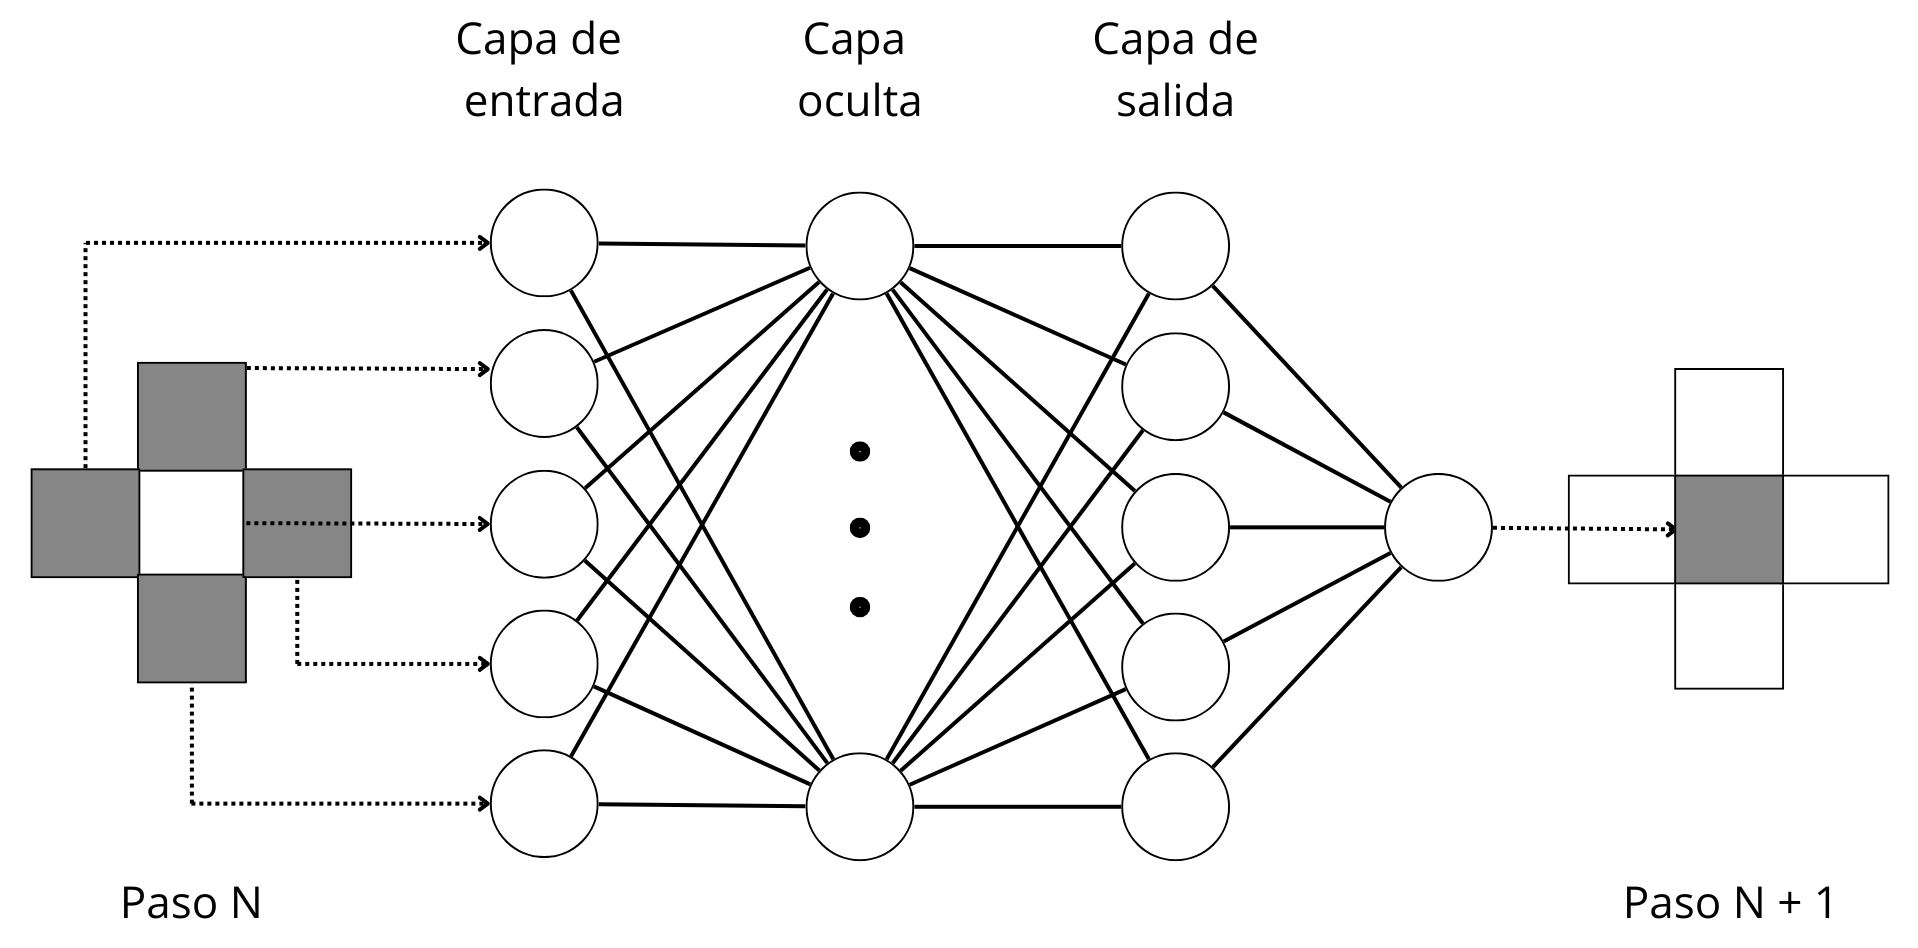
\includegraphics[width=\linewidth]{nca.png}
	\caption{Autómata celular neuronal con vecindad de von Neumann. Los estados de la vecindad en el paso $t$ son la entrada del perceptrón multicapa, cuya salida es el nuevo estado de la célula central en el paso $t+1$.}
	\label{fig:nca}
\end{figure}

En este trabajo, $F_\theta$ es un perceptrón multicapa. Su entrada son los estados de la vecindad, ya sea como números (entrada lineal) o con codificación \onehot{}, en la que cada estado se representa con un vector binario que tiene un solo 1. Esta codificación evita que la red suponga una relación de orden lineal entre estados que no la tienen \cite{MenchacaMendez2022}, por ejemplo, sin ella asume que el estado 2 esté más cerca del 3 que del 9. La capa de salida tiene una neurona por estado y el nuevo estado es el de mayor valor. Para describir la red se usa la notación \red{$L$:$n$:$\varphi$}{$k$:$\psi$}: $L$ capas ocultas de $n$ neuronas con activación $\varphi$ y una capa de salida de $k$ neuronas con activación $\psi$. Por ejemplo, \red{1:4:ReLU}{2:Linear} tiene una capa oculta de 4 neuronas ReLU y dos neuronas de salida lineales.

Como la red es determinista, define una regla local en el sentido de la ecuación~\eqref{eq:regla_local}: basta evaluarla sobre todos los patrones posibles de la vecindad para obtener su vector de regla y compararlo con el de la regla original.

\subsection{Entrenamiento}

Cada célula, en cada paso de la evolución, es una muestra de entrenamiento: la entrada son los estados de su vecindad y la salida esperada es su estado en el paso siguiente. Así, una evolución de $T$ pasos en un espacio de $H \times W$ células aporta $(T-1)\,H\,W$ muestras. Los vecinos que caen fuera del espacio se tratan con frontera periódica o abierta.

La red se entrena con la entropía cruzada como función de pérdida y el optimizador Adam \cite{kingma2015_adam}. La tasa de aprendizaje puede mantenerse constante, reducirse de forma exponencial hasta un valor mínimo o reducirse a la mitad cada vez que la pérdida deja de mejorar durante 20 épocas (reducción por \textit{plateau}). El entrenamiento termina al llegar al número máximo de épocas o cuando la pérdida es menor que la \textit{pérdida objetivo}, que fija qué tan exacta debe ser la regla aprendida.

\subsection{Métricas de evaluación}

Para los sistemas con regla conocida se usan la pérdida, la exactitud de un paso (fracción de células cuyo siguiente estado se predice correctamente) y, en el juego de la vida, la distancia Manhattan entre el vector de la regla original y el de la aprendida.

En los sistemas reales no existe una regla de referencia, por lo que cada red se compara con la predicción sin cambio, que supone que el siguiente paso es igual al actual. Como de un paso a otro cambian pocas células, esta predicción es difícil de superar, pero nunca reproduce la dinámica. Los errores se reportan de forma relativa,
\begin{equation}
	\varepsilon = 100\,\% \cdot \frac{E_{\text{red}}}{E_{\text{sin cambio}}},
	\label{eq:error_relativo}
\end{equation}
de modo que un valor menor que 100\,\% indica que la red mejora a la predicción sin cambio. Además del error de un paso se mide la simulación libre, en la que la red parte de la primera imagen real y evoluciona sola con sus propias predicciones. En FLAME~3 y SEVIR se mide qué tanto se parecen el área quemada o el área con tormenta de la simulación libre a las reales (100\,\% si son idénticas). En \textit{Physarum polycephalum} se usa la coincidencia del plasmodio con
\begin{equation}
	C_t = \frac{|R_t \cap S_t|}{|R_t \cup S_t|} \cdot \frac{\min(|R_t|, |S_t|)}{\max(|R_t|, |S_t|)},
	\label{eq:coincidencia}
\end{equation}
donde $R_t$ y $S_t$ son los conjuntos de células con plasmodio en el paso $t$ de la evolución real y de la simulada. El primer factor mide si el plasmodio está en el mismo lugar y el segundo si hay la misma cantidad; $C_t = 1$ si la simulación es idéntica a la real.

\subsection{Procedimiento experimental}

Los experimentos se dividen en dos series. En la primera, que responde a las preguntas P1 a P3, se entrena el autómata celular neuronal con evoluciones de reglas conocidas (el juego de la vida, la pila de arena y la hormiga de Langton): como la regla original existe, la vecindad correcta determina la transición y la regla aprendida puede compararse con la original. Cada sistema agrega una dificultad: el desbalance de patrones y la vecindad desconocida, un número mayor de estados y la escasez de información. En la segunda serie, que responde a P4, la configuración obtenida se aplica a sistemas reales sin regla conocida y con distinto grado de apertura: la propagación de un incendio (FLAME~3), el movimiento de tormentas (SEVIR) y el crecimiento de moho en una caja de Petri (\textit{Physarum polycephalum}), cada uno con un preprocesamiento propio. La tabla~\ref{tab:experimentos} resume la configuración final de cada experimento. Salvo que se indique otra cosa, se usa una tasa de aprendizaje inicial de 0.001, lotes de 4,096 u 8,192 muestras y la semilla aleatoria 42.

\begin{table*}[!tp]
	\centering
	\small
	\begin{tabularx}{\textwidth}{@{}l c >{\raggedright\arraybackslash}p{2.5cm} >{\raggedright\arraybackslash}X >{\raggedright\arraybackslash}p{4.3cm}@{}}
		\toprule
		\textbf{Sistema} & \textbf{Estados} & \textbf{Vecindad} & \textbf{Datos de entrenamiento} & \textbf{Red seleccionada} \\
		\midrule
		Juego de la vida & 2 & Moore, $3\times3$ (9) & 100 evoluciones aleatorias de B3/S23 en $100\times100$ por 100 pasos & \red{1:4:ReLU}{2:Linear} \\
		Pila de arena & 17 & von Neumann (5) & 2 evoluciones de $25\times25$ durante 2,000 pasos, con 1 y 4 generadoras & \red{2:64:ReLU}{17:Linear}, \onehot{} \\
		Hormiga de Langton & $5n$ (10--50) & Rombo de radio 2 (13) & 2 hormigas en $30\times30$ durante 10,000 pasos, de 2 a 10 colores & \red{4:64:ReLU}{$5n$:Linear}, \onehot{} \\
		FLAME~3 & 18 & $9\times9$ (81) & 1 de 2 secuencias térmicas (116 y 66 imágenes) de $100\times100$ & \red{2:32:ReLU}{18:Linear}, \onehot{}, paso de 30 s \\
		SEVIR & 7 & $11\times11$ (121) & 400 tormentas de 2018, 5 transiciones cada una, $96\times96$ & \red{16:64:ReLU}{7:Linear}, entrada lineal \\
		\textit{Physarum} & 24 & 97 vecinos & 20 cajas de Petri de $160\times160$ células & \red{16:128:ReLU}{24:Linear}, \onehot{} \\
		\bottomrule
	\end{tabularx}
	
	\caption{Resumen de los seis experimentos y de la red seleccionada en cada uno.}
	\label{tab:experimentos}
\end{table*}

	\section{RESULTADOS}
\label{sec:resultados}

En esta sección se presentan los seis experimentos. Los tres primeros replican sistemas con regla conocida y los tres siguientes aplican la configuración obtenida a sistemas reales.

\subsection{El juego de la vida}

Se usó la regla B3/S23 con 100 condiciones iniciales aleatorias de $100 \times 100$ durante 100 pasos, en las que en promedio el 16.5\,\% de las células está viva. Para analizar el desbalance de entradas se usa la nomenclatura $C x N y$, que cuenta las células vivas en el centro ($C$) y en el exterior ($N$) de la vecindad. Como la regla genera poca vida, los patrones $C0N8$ y $C1N8$ suman menos del 0.02\,\% de las vecindades (figura~\ref{fig:gol_patrones}), lo que produce un sesgo de muestra.

\begin{figure}[!tp]
	\centering
	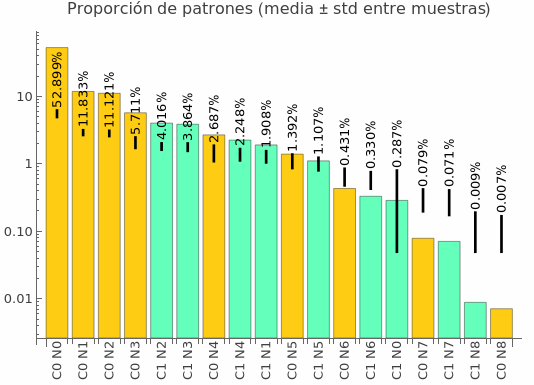
\includegraphics[width=0.85\linewidth]{gol/life_pattern_count.png}
	\caption{Frecuencia de los patrones $C x N y$ en las evoluciones de entrenamiento de la regla B3/S23.}
	\label{fig:gol_patrones}
\end{figure}

\subsubsection{Capacidad de replicación}
Con una pérdida objetivo exigente de $10^{-4}$ se probaron 10 combinaciones de funciones de activación (tabla~\ref{tab:gol_activaciones}). Con una capa oculta de 4 neuronas, únicamente \red{1:4:ReLU}{2:Linear} converge en 122 épocas y con 4 capas de 8 neuronas convergen cinco configuraciones. Las que no convergen se estancan en las primeras 12 épocas, lo que indica un problema de la combinación de activaciones más que de la tasa de aprendizaje; las redes lineales no pueden representar la regla y se quedan en una pérdida de 0.2975.

\begin{table}[!tp]
	\centering
	\footnotesize
	\setlength{\tabcolsep}{3.5pt}
	\begin{tabular}{@{}llrlrl@{}}
		\toprule
		& & \multicolumn{2}{c}{\textbf{1:4}} & \multicolumn{2}{c}{\textbf{4:8}} \\
		\cmidrule(lr){3-4} \cmidrule(l){5-6}
		\textbf{Oculta} & \textbf{Salida} & \textbf{Épocas} & \textbf{Pérdida} & \textbf{Épocas} & \textbf{Pérdida} \\
		\midrule
		ReLU & 2:Linear & \textbf{122} & $\mathbf{9.8\times10^{-5}}$ & 18 & $8.7\times10^{-5}$ \\
		TanH & 1:Sigmoid & 1,000 & 0.0529 & 51 & $9.7\times10^{-5}$ \\
		TanH & 2:Linear & 1,000 & 0.0794 & 35 & $9.7\times10^{-5}$ \\
		Sigmoid & 2:Linear & 1,000 & 0.1593 & 79 & $9.5\times10^{-5}$ \\
		ReLU & 1:Sigmoid & 1,000 & 0.2692 & 133 & $9.6\times10^{-5}$ \\
		Sigmoid & 1:Sigmoid & 1,000 & 0.1593 & 1,000 & 0.1593 \\
		ReLU & 2:TanH & 1,000 & 0.1796 & 1,000 & 0.1269 \\
		Linear & 1:Sigmoid & 1,000 & 0.2975 & 1,000 & 0.2975 \\
		Linear & 2:Linear & 1,000 & 0.2975 & 1,000 & 0.2975 \\
		ReLU & 2:Sigmoid & 1,000 & 0.3748 & 1,000 & 0.3748 \\
		\bottomrule
	\end{tabular}
	\caption{Épocas y pérdida final de B3/S23 con 1 capa oculta de 4 neuronas y con 4 capas de 8. Pérdida objetivo $10^{-4}$, límite de 1,000 épocas, lote de 8,192.}
	\label{tab:gol_activaciones}
\end{table}

\subsubsection{Pérdida objetivo y regla aprendida}
Aunque B3/S23 es semitotalística, la red puede distinguir entre permutaciones de un mismo patrón y aprender una regla arbitraria. Para extraer la regla aprendida se evoluciona un paso un espacio que contiene las 512 configuraciones de la vecindad de Moore y se compara con la regla original (figura~\ref{fig:gol_reglas}):

\begin{itemize}
	\item \textbf{B3/S23} solo aprende dos comportamientos: la regla 0 con pérdidas objetivo de 0.2 y 0.3, y la regla exacta con 0.1 o menos.
	\item \textbf{B3/S238}, con pérdidas objetivo de 0.03 a 0.1, difiere solo en el patrón $C1N8$, que tiene una única representación: la red aprende B3/S23.
	\item \textbf{B38/S238} aprende B3/S238 o B3/S23, según la pérdida objetivo.
	\item \textbf{B3/S236}, con pérdida objetivo de 0.2, cambia las 28 permutaciones de $C1N6$ de 1 a 0 y 4 de las 8 de $C1N7$ de 0 a 1, por lo que la regla aprendida no es semitotalística; con 0.02 a 0.1 aprende B3/S23678.
\end{itemize}

B3/S23 resulta estable, mientras que las reglas que generan vida adicional aprenden otras reglas cuando el entrenamiento es incompleto. Una posible explicación es que la red se inicializa produciendo ceros y, como casi nunca recibe los patrones de baja frecuencia, sus salidas para ellos se mantienen en ese valor.

\begin{figure}[!tp]
	\centering
	\begin{subfigure}[b]{0.49\linewidth}
		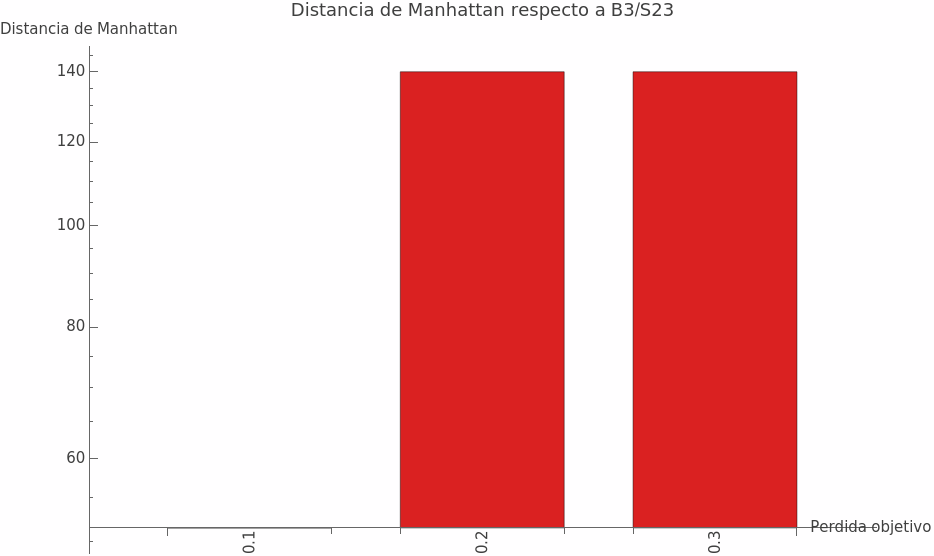
\includegraphics[width=\linewidth]{gol/b3s23_loss.png}
		\caption{B3/S23}
	\end{subfigure}\hfill
	\begin{subfigure}[b]{0.49\linewidth}
		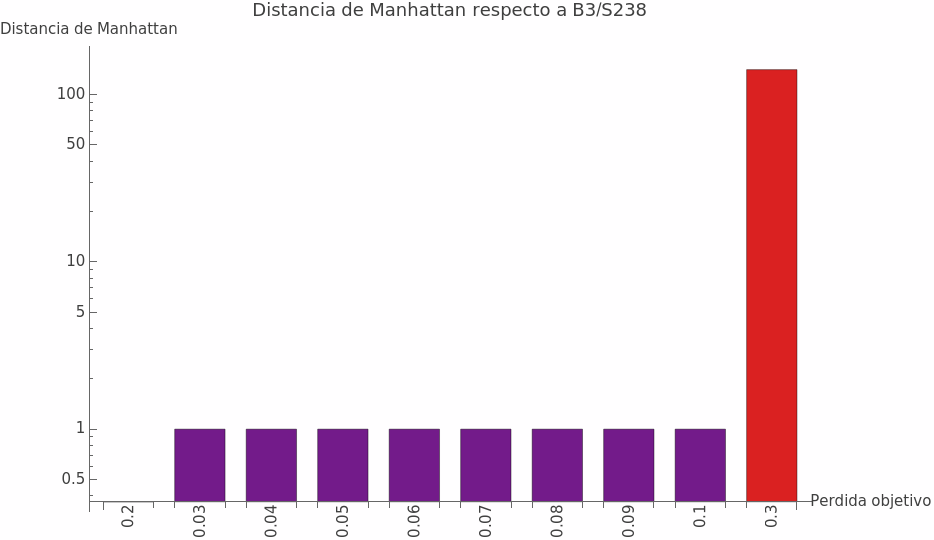
\includegraphics[width=\linewidth]{gol/b3s238_loss.png}
		\caption{B3/S238}
	\end{subfigure}
	\\[4pt]
	\begin{subfigure}[b]{0.49\linewidth}
		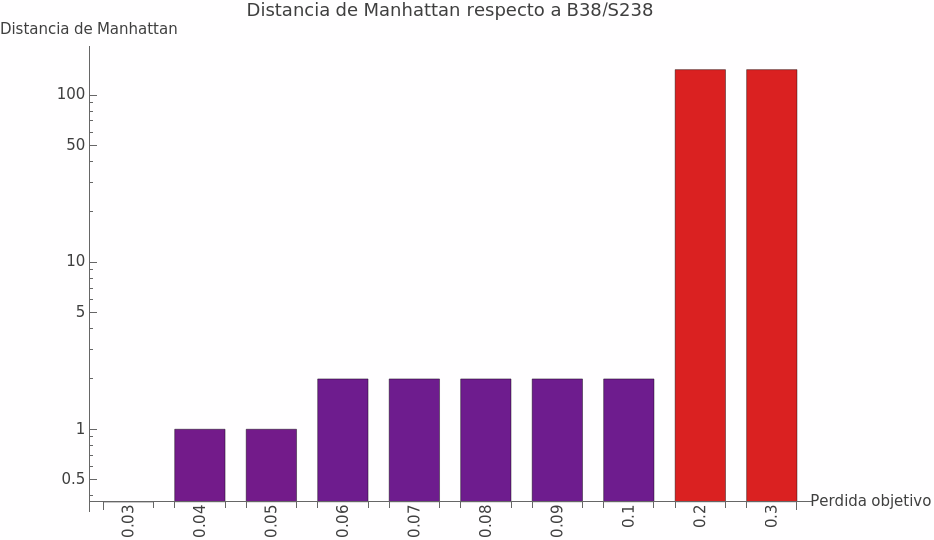
\includegraphics[width=\linewidth]{gol/b38s238_loss.png}
		\caption{B38/S238}
	\end{subfigure}\hfill
	\begin{subfigure}[b]{0.49\linewidth}
		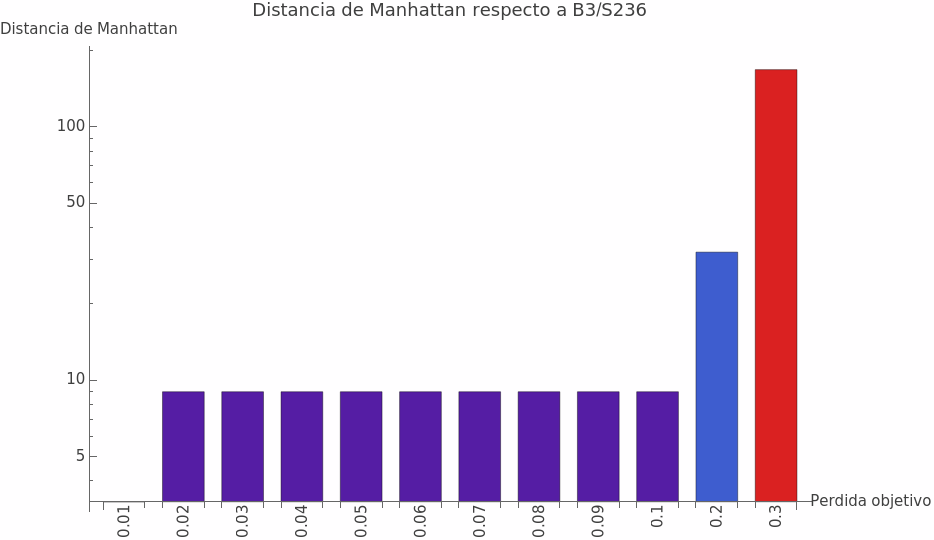
\includegraphics[width=\linewidth]{gol/b3s236_loss.png}
		\caption{B3/S236}
	\end{subfigure}
	\caption{Distancia Manhattan entre el vector de la regla original y el de la regla aprendida con distintas pérdidas objetivo.}
	\label{fig:gol_reglas}
\end{figure}

\subsubsection{Efecto de la vecindad}
En un sistema real la vecindad se desconoce, por lo que se entrenó B3/S23 quitando y agregando vecinos (tabla~\ref{tab:gol_vecindad}). Sin un vecino del exterior la vecindad ya no determina la transición: la pérdida mínima alcanzable es de 0.1213, ninguna red baja de 0.1215 y todas aprenden una regla que difiere en 98 de 512 elementos y solo produce naturaleza muerta. Sin la célula central la pérdida mínima es menor (0.0787), lo que confirma que la transición depende más de los vecinos que del propio estado. En cambio, ampliar la vecindad hasta $8\times8$ la sigue determinando y no impide replicar la regla, mientras que ampliarla sin el vecino faltante reduce la pérdida, pero no a cero.

\begin{table}[!t]
	\centering
	\footnotesize
	\setlength{\tabcolsep}{4pt}
	\begin{tabular}{@{}lll@{}}
		\toprule
		\textbf{Vecindad} & \textbf{Pérdida} & \textbf{Regla aprendida} \\
		\midrule
		$3\times3$ sin $(-1,-1)$ & 0.1215 & Difiere en 98 de 512 elementos \\
		$3\times3$ sin $(0,0)$ & 0.0787 & Extingue casi toda la vida \\
		$5\times5$ & $3.5\times10^{-5}$ & B3/S23 \\
		$7\times7$ & $2.3\times10^{-5}$ & B3/S23 \\
		$8\times8$ & $6.3\times10^{-5}$ & B3/S23 \\
		$9\times9$ sin $(-1,-1)$ & 0.0976 & Parcial \\
		$9\times9$ sin $(0,0)$ & 0.0660 & Parcial \\
		\bottomrule
	\end{tabular}
	\caption{Mejor pérdida final de B3/S23 según la vecindad, entre redes de 1:4 a 16:16 con distintas funciones de activación.}
	\label{tab:gol_vecindad}
\end{table}

\subsection{Pila de arena de Bak--Tang--Wiesenfeld}

En el modelo de pila de arena \cite{bak1987, dhar1999abelian}, una célula generadora agrega un grano en cada paso y, cuando una célula alcanza cuatro granos, los reparte entre sus cuatro vecinos ortogonales. Como el grano que se agrega depende del estado del sistema, no es un autómata celular en sentido estricto. Para representarlo como tal se definen los estados de altura $\mathcal{S}_b = \{0, \dots, 7\}$ y los estados generadores $\mathcal{S}_g = \{0_g, \dots, 8_g\}$, que agregan un grano salvo cuando se derrumban:
\begin{equation*}
	\scriptsize
	\begin{bmatrix} 0 & 4 & 0 \\ 4 & 3_g & 4 \\ 0 & 4 & 0 \end{bmatrix} \!\to\!
	\begin{bmatrix} 2 & 0 & 2 \\ 0 & 8_g & 0 \\ 2 & 0 & 2 \end{bmatrix} \!\to\!
	\begin{bmatrix} 2 & 1 & 2 \\ 1 & 4_g & 1 \\ 2 & 1 & 2 \end{bmatrix} \!\to\!
	\begin{bmatrix} 2 & 2 & 2 \\ 2 & 0_g & 2 \\ 2 & 2 & 2 \end{bmatrix}
\end{equation*}
Con 17 estados y la vecindad de von Neumann, el vector de regla tiene $17^5 = 1{,}419{,}857$ elementos.

\subsubsection{Capacidad de replicación}
Al entrenar con una generadora en el centro, las redes con Sigmoid en las capas ocultas o con Sigmoid o TanH en la salida se quedan en una exactitud de 55.3\,\%, mientras que ReLU en las capas ocultas y Linear en la salida dan los mejores resultados. La tabla~\ref{tab:sp_arquitecturas} muestra que conviene usar más neuronas por capa en lugar de más capas: con \red{2:64:ReLU}{17:Linear} y una pérdida objetivo de $10^{-5}$ se reproduce el 100\,\% de los datos de entrenamiento, y la evolución coincide con la original (figura~\ref{fig:comparaciones}a,b).

\begin{table}[!t]
	\centering
	\footnotesize
	\setlength{\tabcolsep}{3pt}
	\begin{tabular}{@{}lccrrrr@{}}
		\toprule
		& & & & & \multicolumn{2}{c}{\textbf{Exactitud (\%)}} \\
		\cmidrule(l){6-7}
		\textbf{Oculta} & $\boldsymbol{\eta}$ & $\boldsymbol{\mathcal{L}^*}$ & \textbf{Épocas} & \textbf{Pérdida} & \textbf{Total} & \textbf{Gen.} \\
		\midrule
		16:16 & 0.0003 & $10^{-3}$ & 500 & $9.9\times10^{-3}$ & 99.417 & 91.60 \\
		32:32 & 0.001 & $10^{-3}$ & 500 & $1.2\times10^{-2}$ & 99.679 & 89.75 \\
		8:16 & 0.001 & $10^{-4}$ & 1,256 & $8.6\times10^{-5}$ & 99.998 & 99.95 \\
		8:32 & 0.001 & $10^{-4}$ & 476 & $9.3\times10^{-5}$ & 99.996 & 100.00 \\
		4:32 & 0.001 & $10^{-4}$ & 392 & $9.8\times10^{-5}$ & 99.998 & 100.00 \\
		2:64 & 0.001 & $10^{-4}$ & 351 & $9.9\times10^{-5}$ & 99.999 & 100.00 \\
		2:64 & 0.001 & $10^{-5}$ & 630 & $1.0\times10^{-5}$ & \textbf{100.000} & \textbf{100.00} \\
		\bottomrule
	\end{tabular}
	
	\caption{Pila de arena con una generadora, salida 17:Linear y tasa de aprendizaje constante. Exactitud total y en las células generadoras.}
	\label{tab:sp_arquitecturas}
\end{table}

\begin{figure*}[!t]
	\centering
	\begin{subfigure}[b]{0.155\textwidth}
		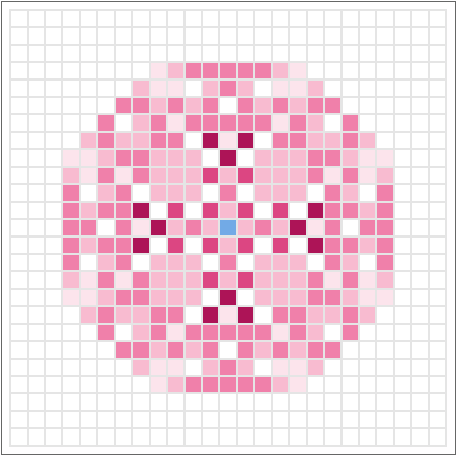
\includegraphics[width=\linewidth]{sandpile/sp_1000.png}
		\caption{Pila, original}
	\end{subfigure}\hfill
	\begin{subfigure}[b]{0.155\textwidth}
		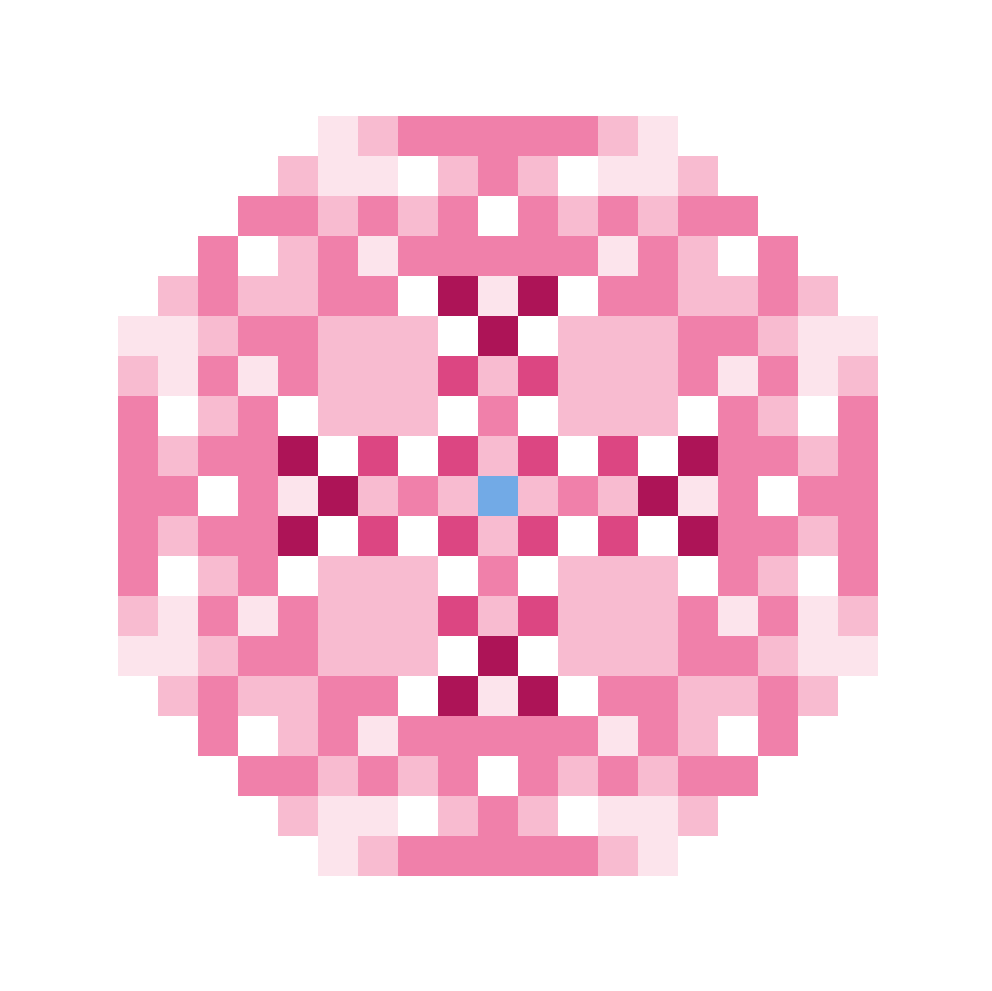
\includegraphics[width=0.93\linewidth]{sandpile/sp_nca_1000.png}
		\caption{Pila, NCA}
	\end{subfigure}\hfill
	\begin{subfigure}[b]{0.155\textwidth}
		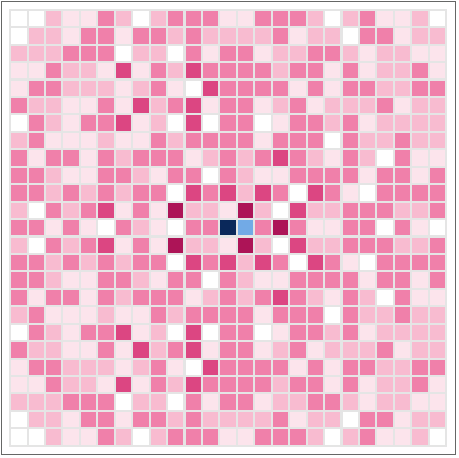
\includegraphics[width=\linewidth]{sandpile/sp_2gen_step_1883.png}
		\caption{Contiguas, original}
	\end{subfigure}\hfill
	\begin{subfigure}[b]{0.155\textwidth}
		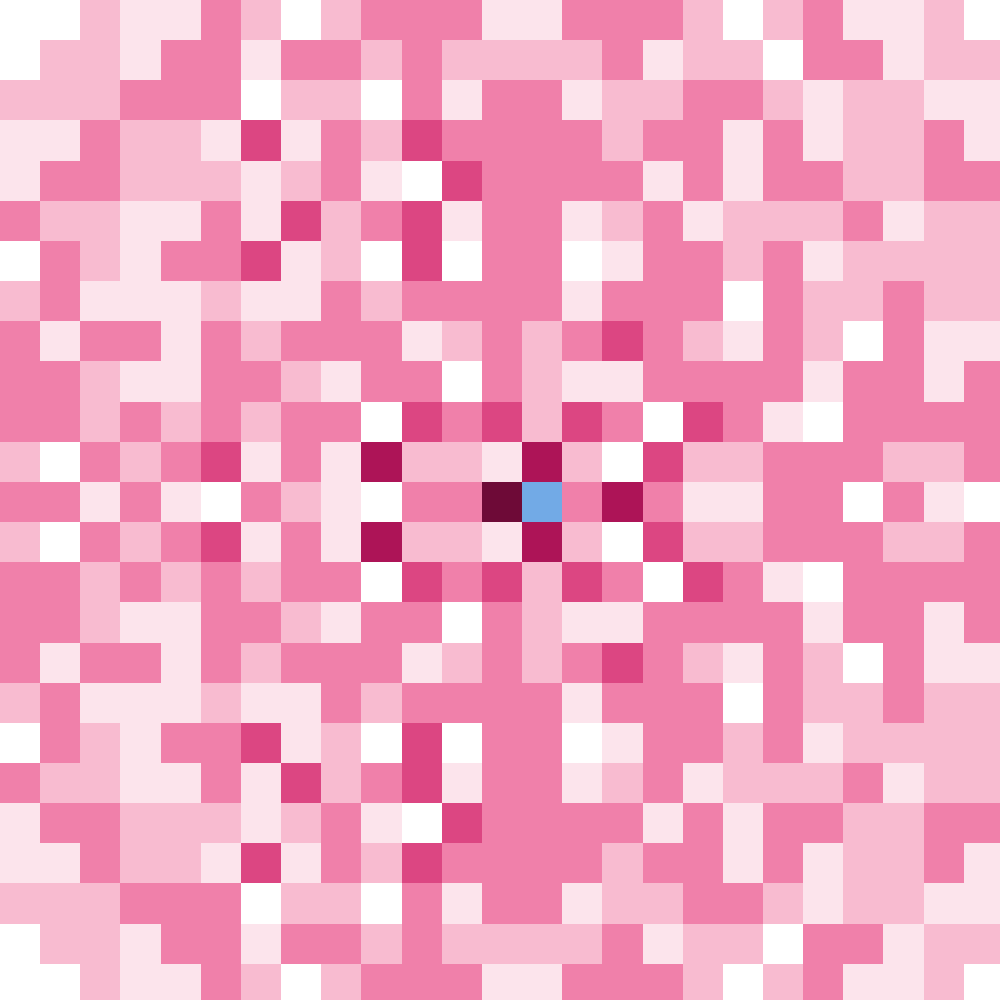
\includegraphics[width=0.96\linewidth]{sandpile/sp_nca_2gen_step_1883.png}
		\caption{Contiguas, NCA}
	\end{subfigure}\hfill
	\begin{subfigure}[b]{0.155\textwidth}
		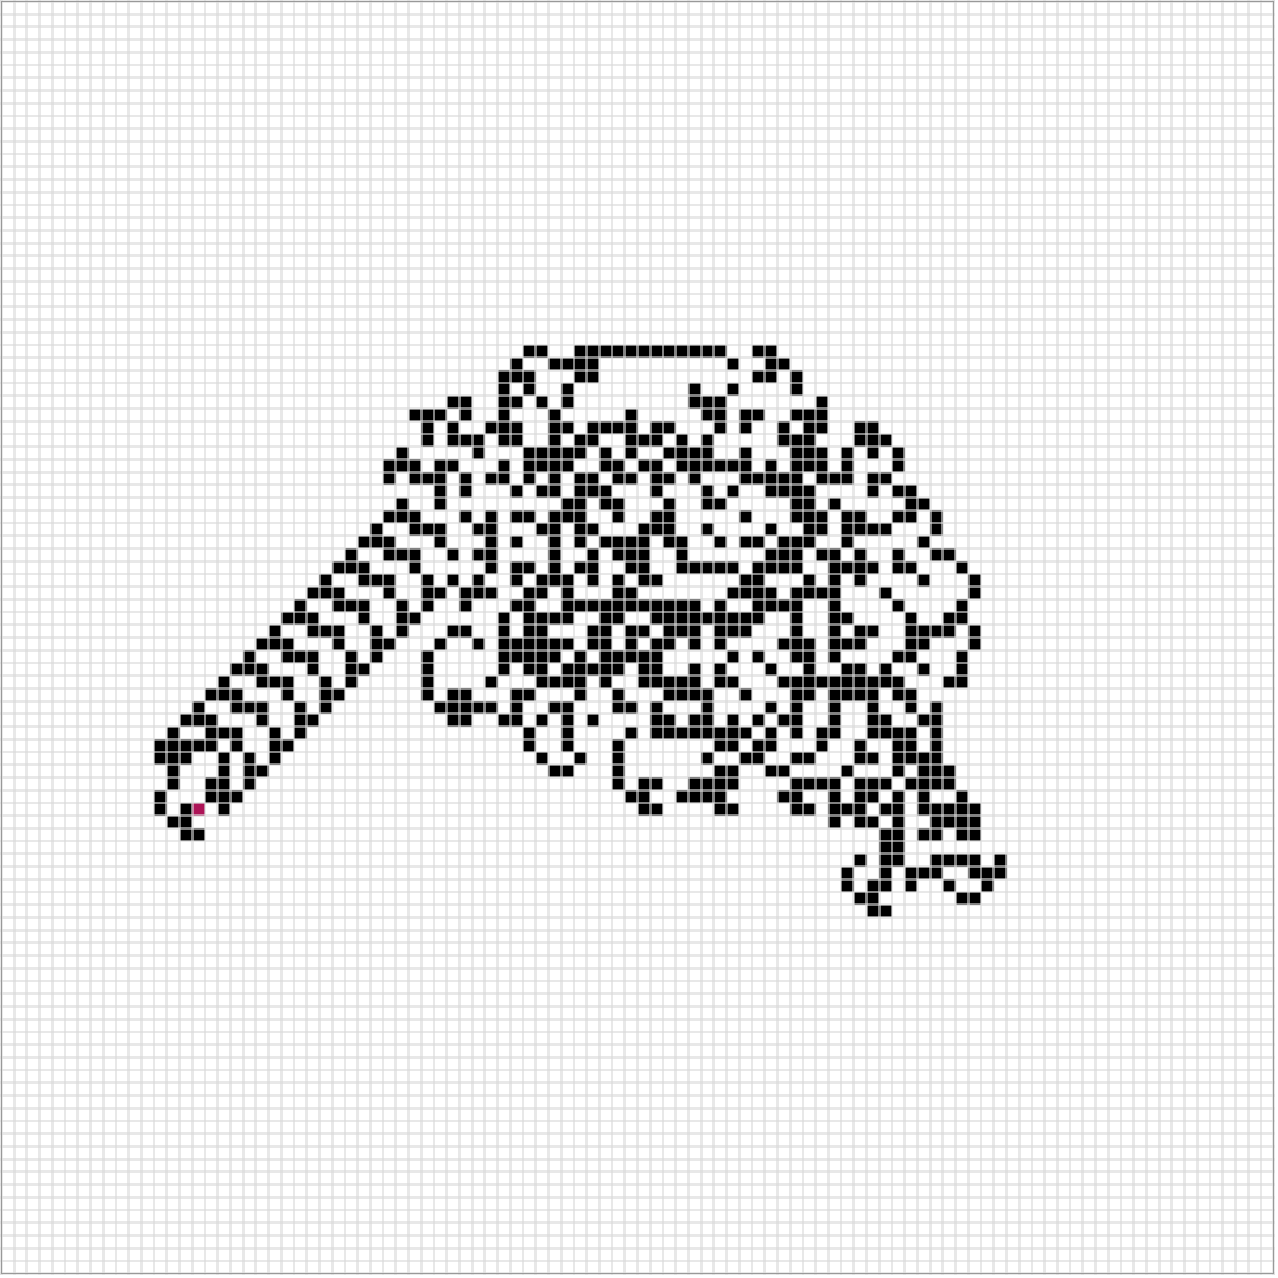
\includegraphics[width=\linewidth]{langton/langton_RL_100x100_paso_11000.png}
		\caption{Hormiga, original}
	\end{subfigure}\hfill
	\begin{subfigure}[b]{0.155\textwidth}
		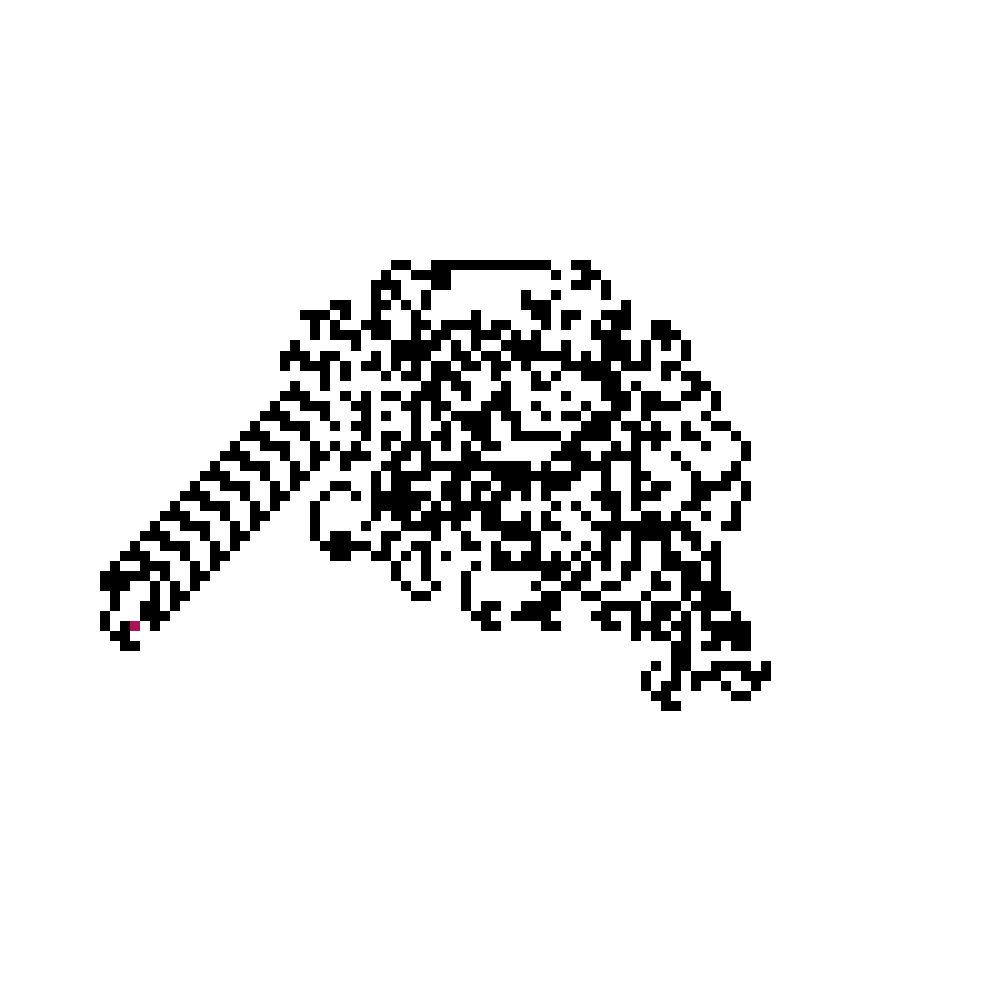
\includegraphics[width=0.96\linewidth]{langton/langton_RL_nca_100x100_paso_11000.png}
		\caption{Hormiga, NCA}
	\end{subfigure}
	\caption{Evolución original, generada en Mathematica, y del autómata celular neuronal (NCA) con la misma configuración inicial. (a, b) Pila de arena con una generadora en el paso 1,000, en tonos azules. (c, d) Dos generadoras contiguas en un espacio de $25\times25$ en el paso 1,883, el primero en el que las evoluciones difieren. (e, f) Hormiga de Langton RL después de 11,000 pasos.}
	\label{fig:comparaciones}
\end{figure*}

\subsubsection{Reducción de la tasa de aprendizaje}
La red entrenada con una generadora no generaliza: con varias generadoras crea nuevas o las elimina. Al entrenar con dos evoluciones de $25 \times 25$ y 2,000 pasos, con una y con cuatro generadoras, estas coexisten, pero la pérdida oscila a partir de la época 150 (figura~\ref{fig:sp_lr}). La reducción exponencial de la tasa de aprendizaje, de 0.001 a $10^{-6}$ en 2,000 épocas, suaviza la curva, pero termina por límite de épocas con una pérdida de $1.5 \times 10^{-5}$, mientras que la reducción por \textit{plateau} alcanza la pérdida objetivo de $10^{-6}$ en 1,319 épocas.

\begin{figure*}[!t]
	\centering
	\begin{subfigure}[b]{0.3\textwidth}
		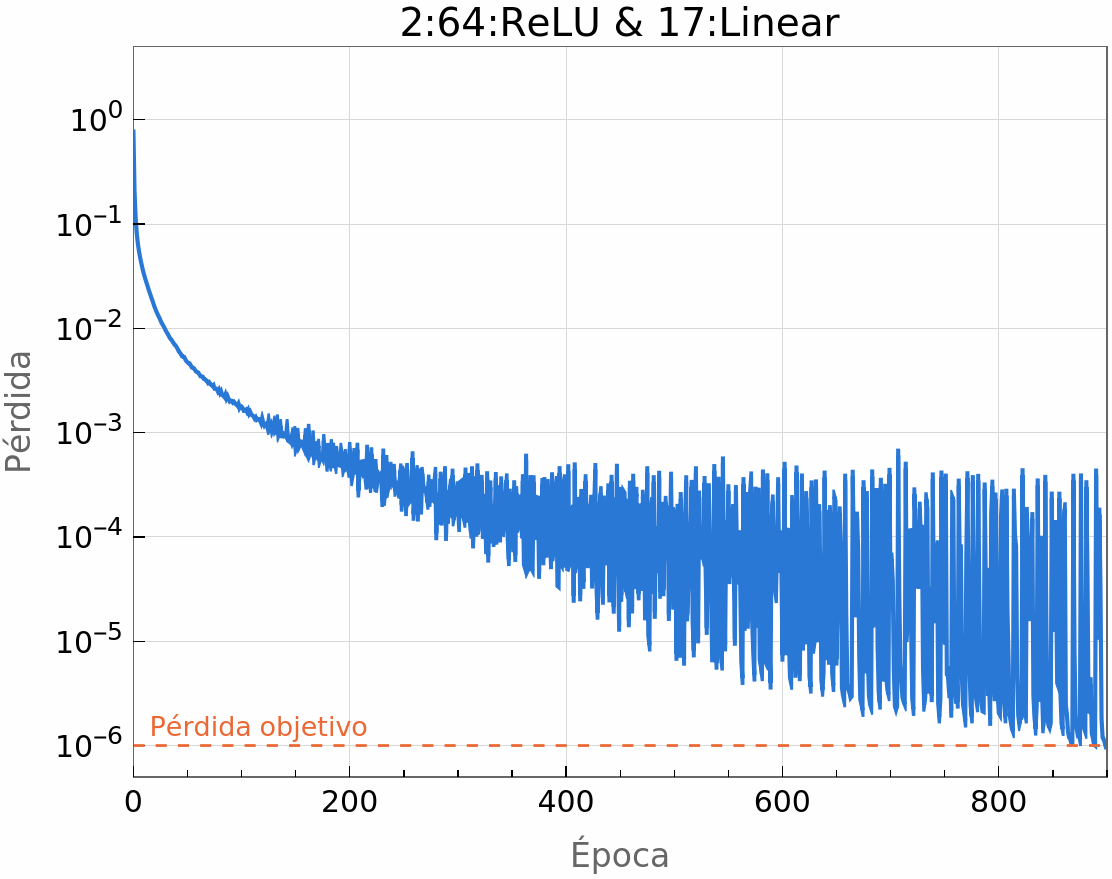
\includegraphics[width=\linewidth]{sandpile/sp_4generadores_loss.png}
		\caption{Tasa constante de 0.001}
	\end{subfigure}\hfill
	\begin{subfigure}[b]{0.3\textwidth}
		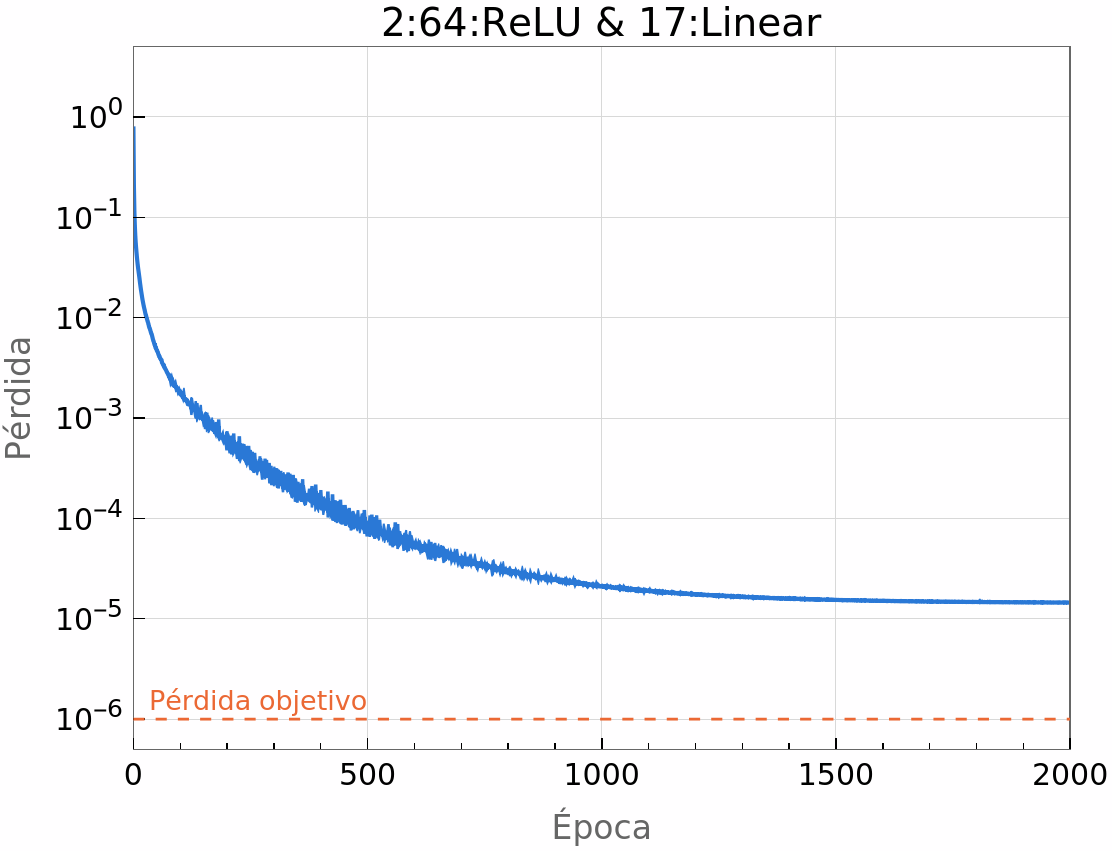
\includegraphics[width=\linewidth]{sandpile/sp_4generadores_loss_exp.png}
		\caption{Reducción exponencial}
	\end{subfigure}\hfill
	\begin{subfigure}[b]{0.3\textwidth}
		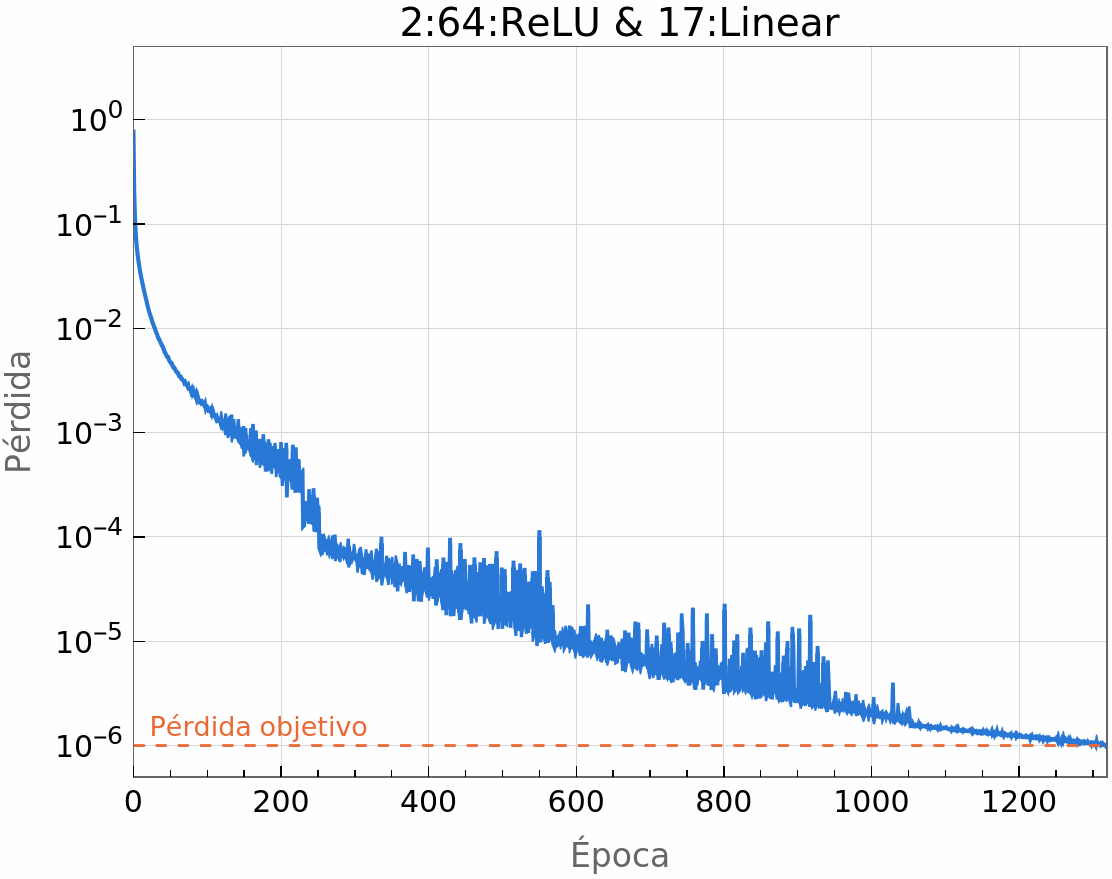
\includegraphics[width=\linewidth]{sandpile/sp_4generadores_loss_plateau.png}
		\caption{Reducción por \textit{plateau}}
	\end{subfigure}
	\caption{Pérdida al entrenar la pila de arena con una y cuatro generadoras y una pérdida objetivo de $10^{-6}$, según la reducción de la tasa de aprendizaje.}
	\label{fig:sp_lr}
\end{figure*}

\subsubsection{Codificación one-hot}
Con la entrada lineal, la red supone que la relación entre los estados 7 y 8 (altura máxima y generadora vacía) es la misma que entre el 0 y el 1. Con \onehot{} la entrada pasa de 5 neuronas con valores de 0 a 16 a 85 neuronas binarias, y con cuatro generadoras la red converge en 63 veces menos épocas y 53 veces menos tiempo (tabla~\ref{tab:sp_onehot}). También mejora la generalización: con una generadora, la evolución conserva su simetría durante 5,149 pasos en lugar de 2,043, y la red entrenada con cuatro generadoras la conserva al menos 10,000 pasos en la configuración tradicional y 2,985 con frontera periódica.

\begin{table}[!t]
	\centering
	\footnotesize
	\setlength{\tabcolsep}{4pt}
	\begin{tabular}{@{}llrrr@{}}
		\toprule
		\textbf{Datos} & \textbf{Entrada} & \textbf{Épocas} & \textbf{Pérdida} & \textbf{Tiempo (s)} \\
		\midrule
		\multirow{2}{*}{1 generadora} & Lineal & 1,200$^\dagger$ & $3\times10^{-6}$ & 140.97 \\
		& \textit{One-hot} & 40 & $1\times10^{-6}$ & 4.92 \\
		\midrule
		\multirow{2}{*}{1 y 4 generadoras} & Lineal & 1,319 & $1\times10^{-6}$ & 301.47 \\
		& \textit{One-hot} & 21 & $1\times10^{-6}$ & 5.67 \\
		\bottomrule
		\multicolumn{5}{@{}l}{\scriptsize $^\dagger$Terminó por límite de épocas.}
	\end{tabular}
	
	\caption{Efecto de la codificación \onehot{} en la pila de arena. Red \red{2:64:ReLU}{17:Linear}, pérdida objetivo $10^{-6}$ y reducción por \textit{plateau}. Todas alcanzan el 100\,\% de exactitud.}
	\label{tab:sp_onehot}
\end{table}

Esta red replicó parcialmente un caso que nunca vio, dos generadoras contiguas: en un espacio de $25\times25$ ambas evoluciones coinciden durante 1,882 pasos (figura~\ref{fig:comparaciones}c,d), hasta que aparece un patrón ausente en el entrenamiento, la generadora con 5 granos junto a otra. En espacios de $20\times20$ y $50\times50$ el primer error aparece en los pasos 1,270 y 6,265, y en $100\times100$ no hay errores en 10,000 pasos.

\subsection{Hormiga de Langton}

La hormiga de Langton es un agente que, sobre una célula de color $i$, gira según la letra $i$ de una cadena (R a la derecha, L a la izquierda), cambia la célula al color $(i+1) \bmod n$ y avanza. Como autómata celular requiere $n + 4n = 5n$ estados ($n$ colores sin hormiga y $4n$ con hormiga en cada dirección), y pone a prueba la extracción de comportamientos con poca información: en cada paso solo cambian dos células.

Para la hormiga RL (10 estados) se usó la vecindad de von Neumann, con un vector de regla de $10^5$ elementos. Con \red{2:8:ReLU}{10:Linear}, \onehot{} y una pérdida objetivo de $10^{-4}$, la red reproduce el comportamiento a la perfección en 36 épocas: tras 11,000 pasos, la evolución es idéntica a la original (figura~\ref{fig:comparaciones}e,f). Con dos hormigas, la red conserva correctamente a las hormigas vecinas que no colisionan, un caso ausente del entrenamiento, y cuando dos hormigas van a ocupar la misma célula elimina una de ellas de forma consistente. Como el modelo original no define este caso, para los siguientes datos se adoptó una regla explícita: si dos hormigas van a colisionar, ambas giran sin avanzar.

Para estudiar el crecimiento del número de estados se generó, para cada número de colores de 2 a 10, una evolución con dos hormigas en $30\times30$ con frontera periódica durante 10,000 pasos. Se usó una vecindad en rombo de radio 2 (13 células), pues una célula necesita saber si otra hormiga a dos células también apunta hacia ella, y la red \red{4:64:ReLU}{$5n$:Linear} con \onehot{}, reducción por \textit{plateau} y pérdida objetivo de $10^{-7}$. El número de estados casi no afecta el entrenamiento (tabla~\ref{tab:langton_colores}): todas las redes convergen en menos de 90 épocas y 100 s. Ocho de las nueve reproducen los 10,000 pasos sin errores; la regla RRRLLL tiene un único error en 9 millones de células, durante una colisión, que hace divergir la evolución en el paso 7,028.

\begin{table}[!t]
	\centering
	\footnotesize
	\setlength{\tabcolsep}{4pt}
	\caption{Hormiga de Langton con dos hormigas de 2 a 10 colores en $30\times30$ durante 10,000 pasos.}
	\label{tab:langton_colores}
	\begin{tabular}{@{}cclrlr@{}}
		\toprule
		\textbf{Colores} & \textbf{Estados} & \textbf{Regla} & \textbf{Épocas} & \textbf{Pérdida} & \textbf{Tiempo} \\
		\midrule
		2 & 10 & RL & 22 & $5.18\times10^{-8}$ & 25.6 s \\
		3 & 15 & RLL & 63 & $3.83\times10^{-8}$ & 73.8 s \\
		4 & 20 & RLLR & 16 & $3.27\times10^{-8}$ & 20.0 s \\
		5 & 25 & RLRLL & 44 & $7.81\times10^{-8}$ & 51.3 s \\
		6 & 30 & RRRLLL & 68 & $4.35\times10^{-8}$ & 75.4 s \\
		7 & 35 & RLRLRLL & 77 & $6.77\times10^{-9}$ & 85.7 s \\
		8 & 40 & RLRLRLRR & 63 & $1.57\times10^{-8}$ & 70.4 s \\
		9 & 45 & RLRLRLLRL & 63 & $2.31\times10^{-8}$ & 73.7 s \\
		10 & 50 & RLRLRLRRRL & 87 & $2.38\times10^{-9}$ & 97.3 s \\
		\bottomrule
	\end{tabular}
\end{table}

Sin embargo, reproducir la evolución de entrenamiento no implica haber aprendido la regla completa, que es el problema de cobertura de la sección~\ref{sec:formulacion}. Con la red de 10 colores, una sola hormiga en un espacio de $100\times100$ evoluciona sin errores hasta el paso 12,455, en el que se divide en dos: la célula que deja no cambia de color y conserva una hormiga girada, como si hubiera estado bloqueada. La red aplica la regla de colisión aprendida con dos hormigas a un patrón que nunca vio.

\subsubsection{Configuración recomendada}
De los tres experimentos con regla conocida se obtienen las siguientes recomendaciones:

\begin{itemize}
	\item Usar ReLU en las capas ocultas y Linear en la salida, con pocas capas y más neuronas por capa.
	\item Codificar la entrada en \onehot{} cuando hay más de dos estados; es la mejora que más acelera el entrenamiento y la generalización.
	\item Reducir la tasa de aprendizaje por \textit{plateau} cuando la pérdida oscila.
	\item Usar una vecindad que contenga a todos los vecinos que influyen en la transición; una vecindad mayor no impide aprender la regla.
	\item Usar una pérdida objetivo exigente, pues con un entrenamiento incompleto la pérdida objetivo determina la regla aprendida.
\end{itemize}

\subsection{Propagación de fuego (FLAME~3)}

FLAME~3 \cite{hopkins2024flame3datasetunleashing} contiene imágenes térmicas radiométricas con vista cenital, tomadas con un dron durante la quema controlada de Hanna Hammock en 2023. Se usaron dos secuencias que registran la temperatura de cada píxel cada 5 s: \texttt{flame\_plot\_1}, con 116 imágenes en las que el fuego pasa de cubrir el 2 al 86\,\% del espacio, y \texttt{flame\_plot\_2}, con 66 imágenes en las que pasa del 4 a casi el 100\,\%. Ambas inician con el fuego presente, para que la red no infiera combustión espontánea.

\subsubsection{Preprocesamiento}
El viento desplaza el dron varios píxeles, por lo que cada imagen se alineó con la primera mediante correlación de fase con precisión de 1/20 de píxel, comparando solo el suelo frío entre imágenes separadas por 1, 2, 4, \dots, 128 posiciones y resolviendo la posición de cada una mediante mínimos cuadrados robustos (pérdida de Huber); la corrección máxima fue de 7.69 píxeles. Después se recortó el mayor cuadrado sin bordes vacíos, se redujo a $100\times100$ células y se discretizó en 18 estados (figura~\ref{fig:flame_limpieza}): 12 de temperatura, $\mathcal{S}_b = \{0, \dots, 11\}$, en escala logarítmica entre 25.3 y 604.6\,°C, y 6 de quemado, $\mathcal{S}_q = \{12, \dots, 17\}$. Sea $\tau_{\vec{i}}(t)$ el estado de temperatura de la célula, $T_{\vec{i}}(t)$ su temperatura y $m_{\vec{i}}$ la mínima registrada desde que se quemó; el estado se asigna como
\begin{equation}
	\sigma_{\vec{i}}(t+1) \in
	\begin{cases}
		\mathcal{S}_q & \text{si } \tau_{\vec{i}}(t+1) < \tau_{\vec{i}}(t), \\
		\mathcal{S}_b & \text{si } \sigma_{\vec{i}}(t) \in \mathcal{S}_q \text{ y } T_{\vec{i}}(t+1) > m_{\vec{i}} + 30\,^\circ\mathrm{C}, \\
		\text{el de } \sigma_{\vec{i}}(t) & \text{en otro caso},
	\end{cases}
	\label{eq:flame_estados}
\end{equation}
donde una célula en $\mathcal{S}_b$ toma el estado $\tau_{\vec{i}}(t+1)$ y una en $\mathcal{S}_q$ toma $12 + \lfloor \tau_{\vec{i}}(t+1)/2 \rfloor$. Es decir, una célula que se enfría queda quemada y solo regresa a un estado de temperatura si vuelve a calentarse más de 30\,°C sobre su mínimo. Así, la red puede distinguir el terreno que todavía puede arder del que ya se quemó; agrupar los estados de quemado y usar el umbral de 30\,°C reduce de 28,537 a 9,102 los regresos de quemado a no quemado, causados principalmente por ruido. Esta definición fue la última de varias pruebas: segmentar con \textit{k-means}, usar hasta 50 estados, rotar las imágenes, agregar el combustible como estado fijo o marcar el quemado con un umbral fijo de temperatura no mejoraron la simulación libre o la hacían divergir.

\begin{figure*}[!t]
	\centering
	\begin{subfigure}[b]{0.235\textwidth}
		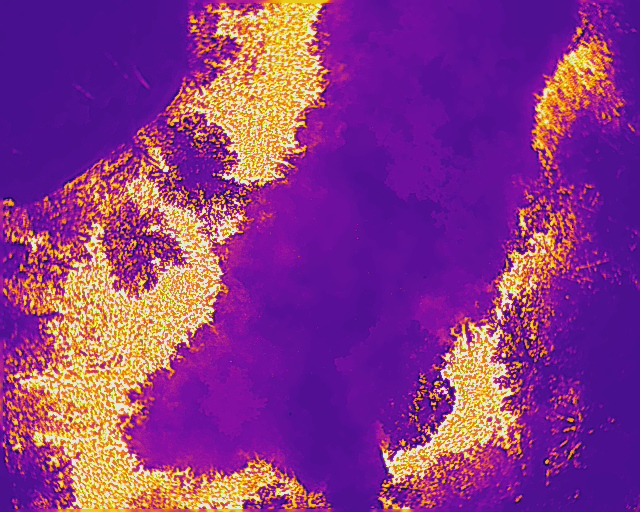
\includegraphics[width=\linewidth]{flame/clean_01.jpg}
		\caption{Imagen original}
	\end{subfigure}\hfill
	\begin{subfigure}[b]{0.235\textwidth}
		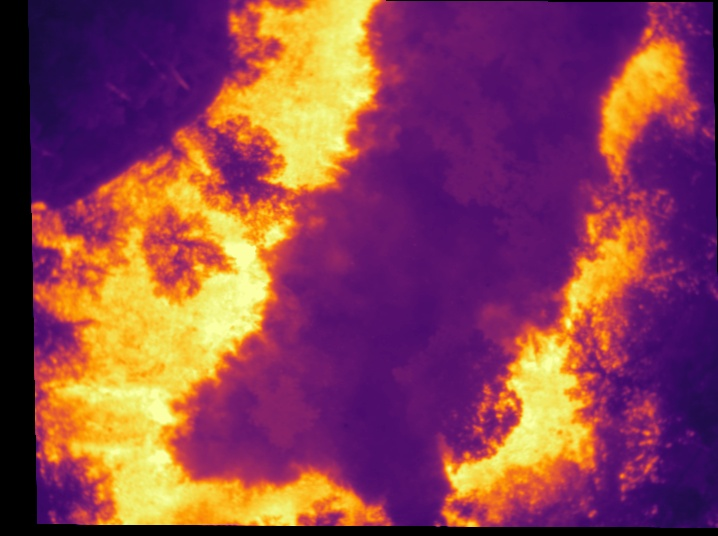
\includegraphics[width=\linewidth]{flame/clean_02.jpg}
		\caption{Alineación}
	\end{subfigure}\hfill
	\begin{subfigure}[b]{0.16\textwidth}
		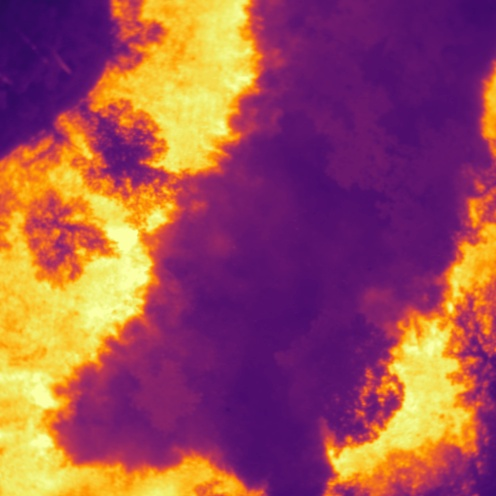
\includegraphics[width=\linewidth]{flame/clean_03.jpg}
		\caption{Recorte}
	\end{subfigure}\hfill
	\begin{subfigure}[b]{0.16\textwidth}
		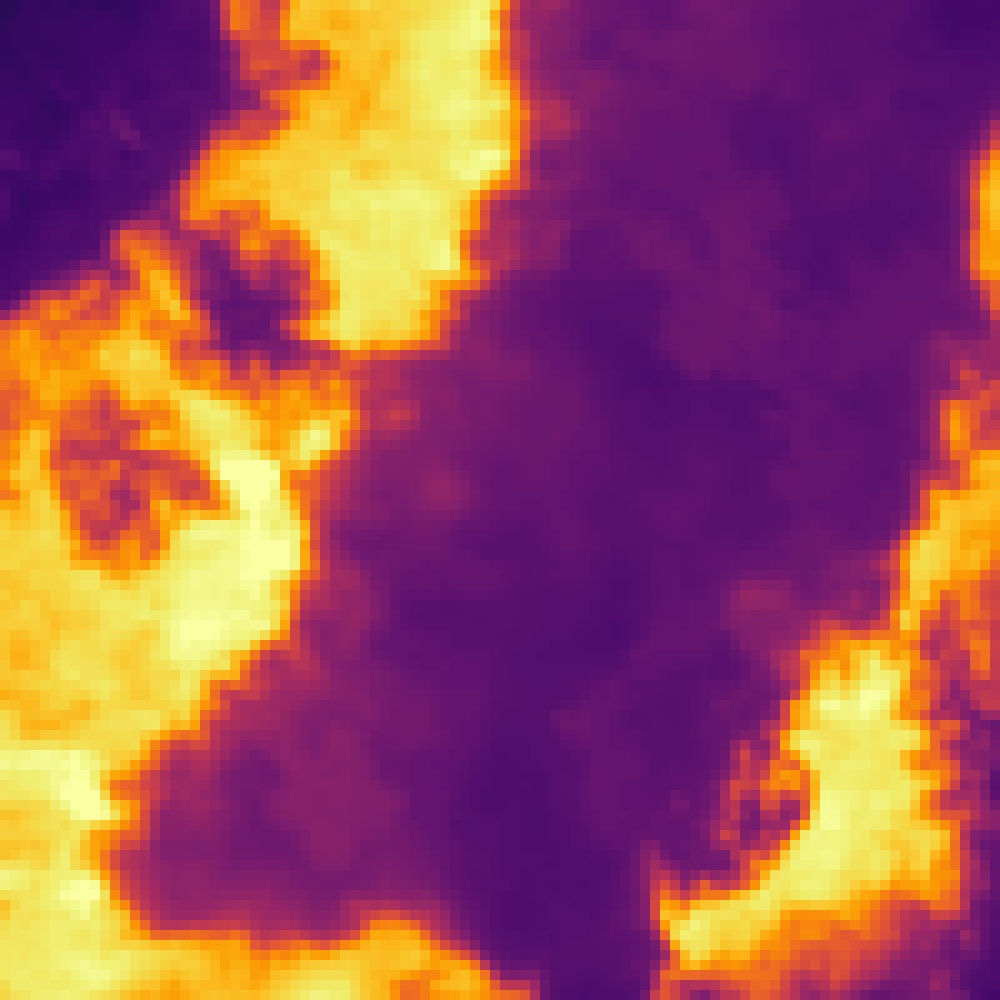
\includegraphics[width=\linewidth]{flame/clean_04.jpg}
		\caption{$100\times100$}
	\end{subfigure}\hfill
	\begin{subfigure}[b]{0.16\textwidth}
		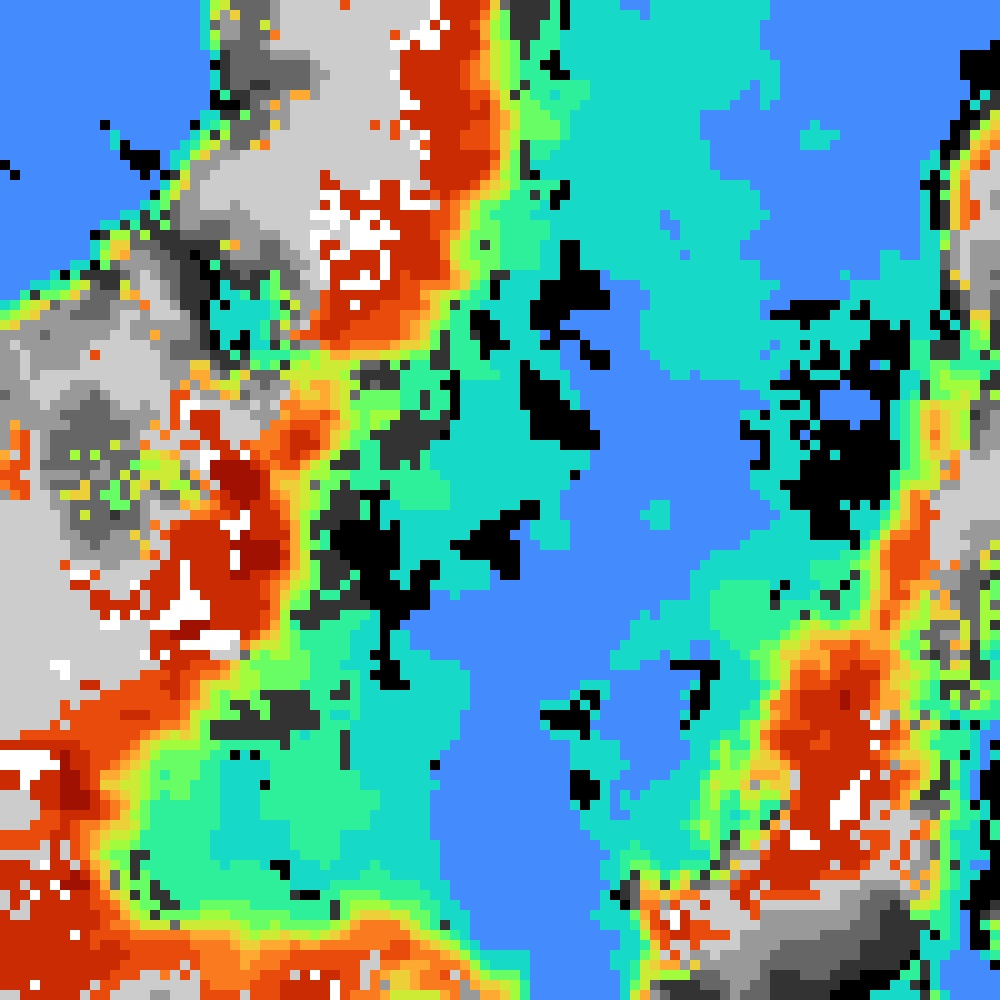
\includegraphics[width=\linewidth]{flame/clean_05_18estados.jpg}
		\caption{18 estados}
	\end{subfigure}
	\caption{Preprocesamiento de la imagen 1204 del \textit{plot} 2 de FLAME~3.}
	\label{fig:flame_limpieza}
\end{figure*}

\subsubsection{Configuraciones y evaluación}
Se probaron 18 configuraciones: paso de 5, 15 o 30 s; vecindad de $9\times9$ (81 vecinos) o dispersa (41 vecinos: el cuadrado de $5\times5$ más 16 células a distancia 5), y capas ocultas 2:32, 3:64 o 4:256 con ReLU, salida 18:Linear y \onehot{}. Se entrenaron 200 épocas con reducción exponencial de 0.001 a $10^{-5}$ y frontera abierta. Cada configuración se entrenó con una secuencia y se probó en la otra en simulación libre, midiendo el área quemada, el área con fuego (células que alcanzan 130\,°C) y los errores de un paso y de la simulación libre relativos a la predicción sin cambio, cuya área quemada es de 0\,\% porque nunca propaga el fuego.

\begin{table}[!t]
	\centering
	\footnotesize
	\setlength{\tabcolsep}{2.5pt}
	\caption{Configuraciones destacadas de FLAME~3. Prueba 1: entrenada con \texttt{flame\_plot\_2} y probada en \texttt{flame\_plot\_1}; prueba 2: al revés. $\varepsilon$: error en la simulación libre relativo a la predicción sin cambio. Lugar: promedio del lugar combinado de las cuatro medidas entre las 18 configuraciones.}
	\label{tab:flame}
	\begin{tabular}{@{}cccrrrrc@{}}
		\toprule
		& & & \multicolumn{2}{c}{\textbf{Prueba 1}} & \multicolumn{2}{c}{\textbf{Prueba 2}} & \\
		\cmidrule(lr){4-5} \cmidrule(lr){6-7}
		& & & \textbf{Área} & & \textbf{Área} & & \\
		\textbf{Paso} & \textbf{Vecindad} & \textbf{Capas} & \textbf{quem.} & $\boldsymbol{\varepsilon}$ & \textbf{quem.} & $\boldsymbol{\varepsilon}$ & \textbf{Lugar} \\
		\midrule
		30 s & $9\times9$ & 2:32 & 85\,\% & 147\,\% & 30\,\% & \textbf{97\,\%} & \textbf{5.5} \\
		30 s & Dispersa & 3:64 & 86\,\% & 140\,\% & 33\,\% & 101\,\% & \textbf{5.5} \\
		15 s & Dispersa & 3:64 & \textbf{86\,\%} & 404\,\% & 40\,\% & 112\,\% & \textbf{5.5} \\
		15 s & $9\times9$ & 3:64 & 85\,\% & 391\,\% & 43\,\% & 99\,\% & 6 \\
		5 s & Dispersa & 4:256 & 83\,\% & 709\,\% & 61\,\% & \textbf{77\,\%} & 6.25 \\
		15 s & $9\times9$ & 4:256 & 79\,\% & 326\,\% & \textbf{67\,\%} & 89\,\% & 7.5 \\
		\bottomrule
	\end{tabular}
\end{table}

\subsubsection{Resultados}
Al probar en \texttt{flame\_plot\_1}, todas las configuraciones propagan el fuego, con un área quemada entre 72 y 86\,\% similar a la real, pero ninguna supera a la predicción sin cambio en la simulación libre: con paso de 30 s se equivocan entre 1.4 y 2.3 veces más, y con 15 s, entre 3.6 y 4.5 veces más. Es decir, el fuego avanza hacia las zonas correctas, pero las temperaturas no coinciden. Al probar en \texttt{flame\_plot\_2} el área quemada llega como máximo al 67\,\%, las mejores son las redes de 4:256 y varias superan a la predicción sin cambio, mientras que las de 2:32 propagan el fuego demasiado lento.

Ninguna configuración es la mejor en ambas pruebas (tabla~\ref{tab:flame}). Tres empatan en el mejor lugar combinado; se eligió la de paso de 30 s, vecindad de $9\times9$ y \red{2:32:ReLU}{18:Linear} por ser la red más pequeña y la única de las tres que, en la prueba 2, se equivoca menos que la predicción sin cambio tanto en un paso (89\,\%) como en la simulación libre (97\,\%). La evaluación visual coincide con el área quemada y verifica que el fuego se propaga a velocidad constante, que los frentes se extinguen al colisionar, que el terreno quemado no vuelve a encenderse y que el sistema se calienta y se enfría (figuras~\ref{fig:flame_criterios} y \ref{fig:flame_comparacion}).

\begin{figure*}[!t]
	\centering
	\begin{subfigure}[t]{0.155\textwidth}
		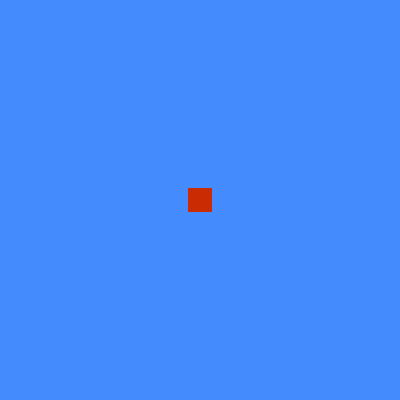
\includegraphics[width=\linewidth]{flame/criterios/paso_0.png}
		\caption{0 s}
	\end{subfigure}\hfill
	\begin{subfigure}[t]{0.155\textwidth}
		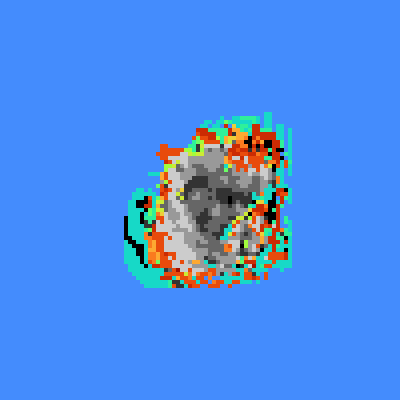
\includegraphics[width=\linewidth]{flame/criterios/paso_5.png}
		\caption{150 s}
	\end{subfigure}\hfill
	\begin{subfigure}[t]{0.155\textwidth}
		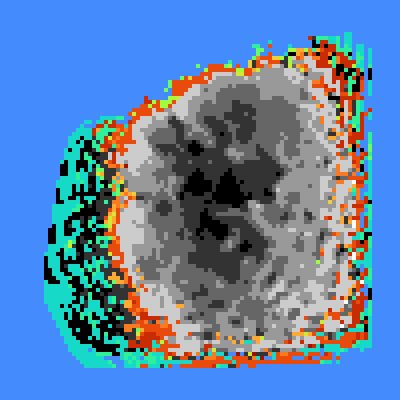
\includegraphics[width=\linewidth]{flame/criterios/paso_10.png}
		\caption{300 s}
	\end{subfigure}\hfill
	\begin{subfigure}[t]{0.155\textwidth}
		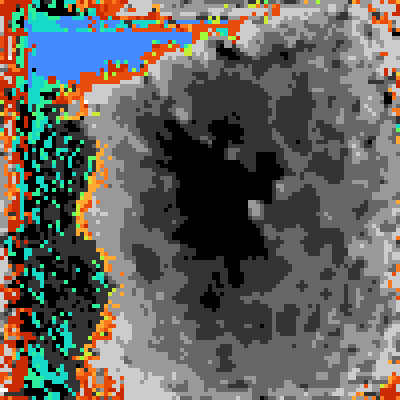
\includegraphics[width=\linewidth]{flame/criterios/paso_14.png}
		\caption{420 s}
	\end{subfigure}\hfill
	\begin{subfigure}[t]{0.155\textwidth}
		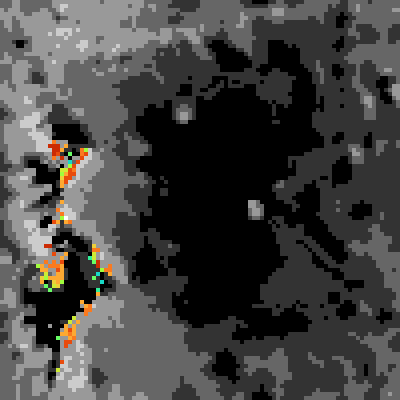
\includegraphics[width=\linewidth]{flame/criterios/paso_18.png}
		\caption{540 s}
	\end{subfigure}\hfill
	\begin{subfigure}[t]{0.155\textwidth}
		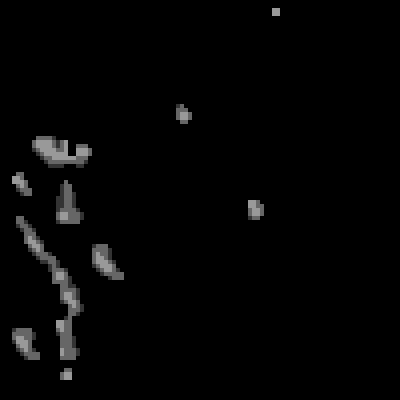
\includegraphics[width=\linewidth]{flame/criterios/paso_40.png}
		\caption{1200 s}
	\end{subfigure}
	\leyendaflame
	\caption{Simulación libre de la configuración final de FLAME~3 con frontera periódica, a partir de un foco de $6\times6$ células en el estado 10 en un espacio frío de $100\times100$. El fuego se propaga en todas direcciones (b, c), los frentes se extinguen al encontrarse tras cruzar la frontera (d, e) y, una vez quemado el espacio, no vuelve a aparecer fuego (f).}
	\label{fig:flame_criterios}
\end{figure*}

\begin{figure}[!t]
	\centering
	\setlength{\tabcolsep}{1pt}
	\begin{tabular}{@{}r@{\hspace{3pt}}ccc@{}}
		& \scriptsize 150 s & \scriptsize 300 s & \scriptsize 420 s \\
		\rotatebox{90}{\scriptsize\quad Real 1} &
		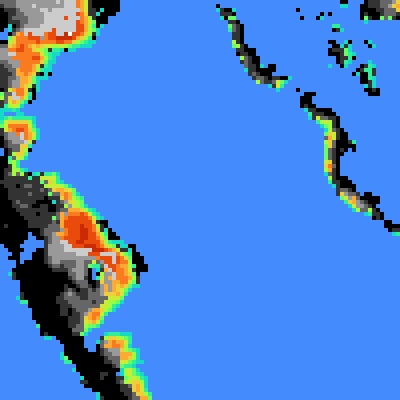
\includegraphics[width=0.28\linewidth]{flame/comparacion/p1_real_150s.png} &
		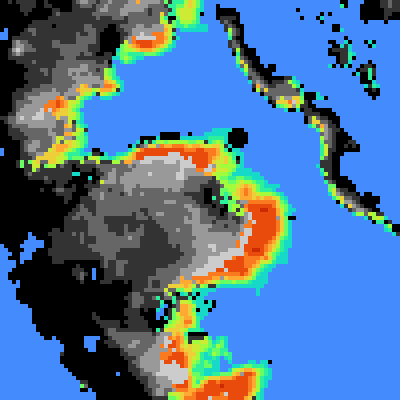
\includegraphics[width=0.28\linewidth]{flame/comparacion/p1_real_300s.png} &
		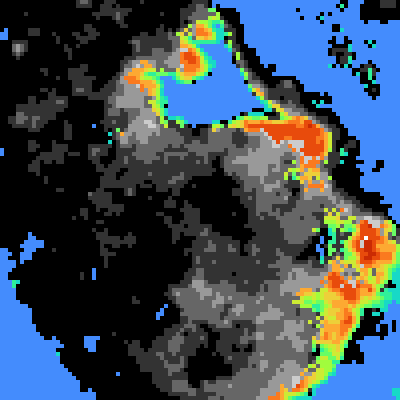
\includegraphics[width=0.28\linewidth]{flame/comparacion/p1_real_420s.png} \\
		\rotatebox{90}{\scriptsize\quad NCA 1} &
		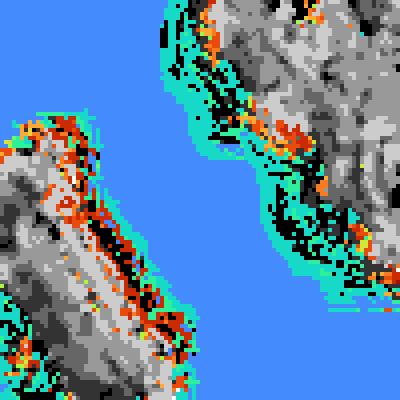
\includegraphics[width=0.28\linewidth]{flame/comparacion/p1_nca_150s.png} &
		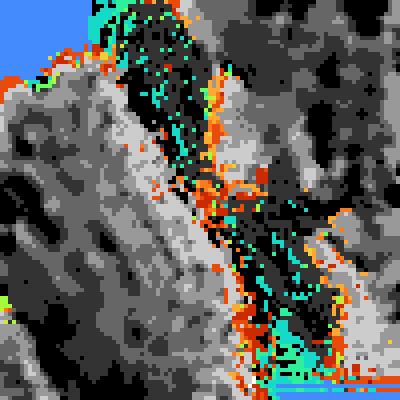
\includegraphics[width=0.28\linewidth]{flame/comparacion/p1_nca_300s.png} &
		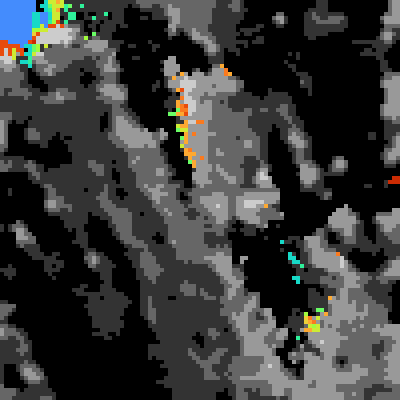
\includegraphics[width=0.28\linewidth]{flame/comparacion/p1_nca_420s.png} \\[2pt]
		& \scriptsize 90 s & \scriptsize 150 s & \scriptsize 240 s \\
		\rotatebox{90}{\scriptsize\quad Real 2} &
		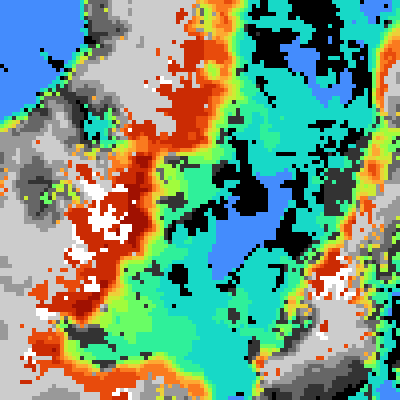
\includegraphics[width=0.28\linewidth]{flame/comparacion/p2_real_90s.png} &
		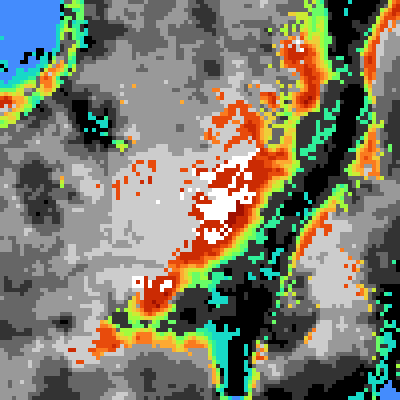
\includegraphics[width=0.28\linewidth]{flame/comparacion/p2_real_150s.png} &
		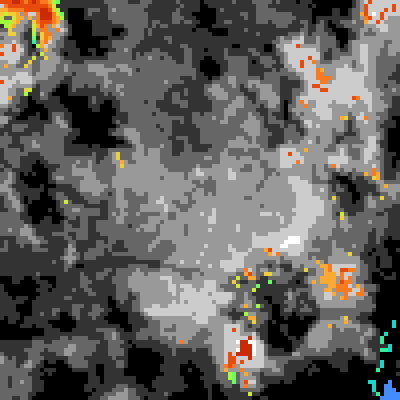
\includegraphics[width=0.28\linewidth]{flame/comparacion/p2_real_240s.png} \\
		\rotatebox{90}{\scriptsize\quad NCA 2} &
		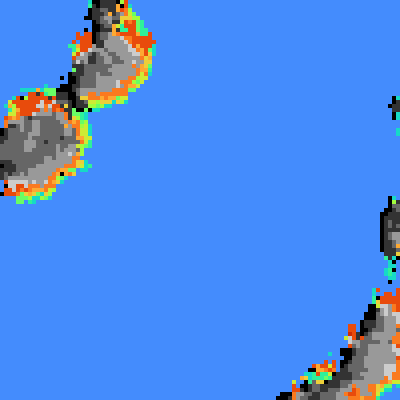
\includegraphics[width=0.28\linewidth]{flame/comparacion/p2_nca_90s.png} &
		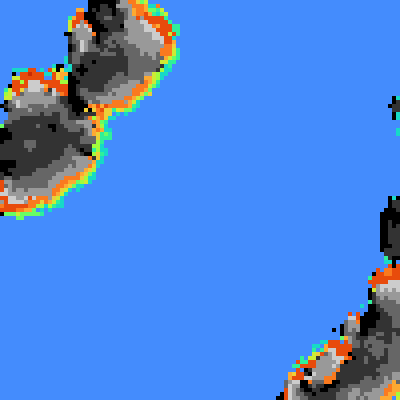
\includegraphics[width=0.28\linewidth]{flame/comparacion/p2_nca_150s.png} &
		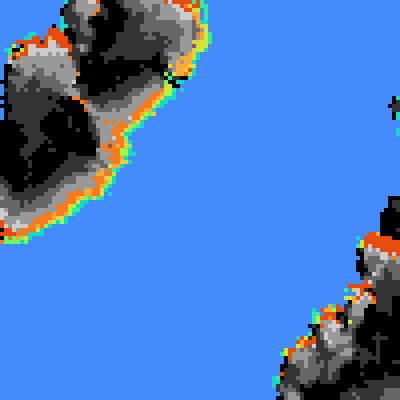
\includegraphics[width=0.28\linewidth]{flame/comparacion/p2_nca_240s.png} \\
	\end{tabular}
	\leyendaflamecorta
	\caption{Evolución real de \texttt{flame\_plot\_1} y \texttt{flame\_plot\_2} y simulación libre de la configuración final entrenada con la otra secuencia.}
	\label{fig:flame_comparacion}
\end{figure}

El experimento está limitado por los datos: FLAME~3 es uno de los pocos conjuntos que registran la propagación con vista cenital y solo aporta dos secuencias cortas con comportamientos distintos, ya que en \texttt{flame\_plot\_1} el terreno permanece frío hasta que llega el fuego y en \texttt{flame\_plot\_2} primero se propagan las temperaturas medias. Además, el modelo ignora el relieve, la vegetación, las carreteras, el viento y la humedad, por lo que la dirección y la velocidad aprendidas dependen de las condiciones de grabación.

\subsection{Movimiento de tormentas (SEVIR)}

SEVIR \cite{veillette2020sevir} contiene más de 10,000 eventos meteorológicos registrados en Estados Unidos entre 2017 y 2019, cada uno con 49 imágenes de $384\times384$ km tomadas cada 5 minutos. Se usaron las imágenes de líquido integrado verticalmente (VIL), reducidas a $96\times96$ células de 4 km, con las que una tormenta avanza alrededor de una célula por paso, y discretizadas con los 6 umbrales que proponen los autores (16, 74, 133, 160, 181 y 219 en la escala de 0 a 255) en 7 estados; una célula tiene tormenta si su estado es 2 o mayor. Se usaron eventos con al menos 2\,\% de tormenta en la primera imagen y frontera abierta, ya que con frontera periódica la red aprendería que las tormentas que entran por el borde aparecen de la nada.

\subsubsection{Capacidad de replicación}
Cuatro configuraciones iniciales ($5\times5$ o $9\times9$, 2:32 o 3:64, \onehot{}), entrenadas con 40 tormentas de 2018 y probadas en 20 de 2019, superan por poco a la predicción sin cambio: aciertan entre el 89.30 y el 89.37\,\% de las células en un paso, contra el 87.64\,\%. Sin embargo, su simulación libre no se parece a una tormenta real (figura~\ref{fig:sevir_comp}): las tormentas se desplazan, pero en pocos pasos se suavizan en manchas uniformes, las células intensas se unen en bloques inmóviles y nunca se forman tormentas nuevas. Mientras que en los datos reales el área con tormenta crece del 12.3 al 19.7\,\% del espacio en 4 horas, en la simulación libre se reduce al 9 o 10\,\%. Como la vecindad no determina la transición, la mejor regla determinista elige en cada célula el estado más probable, que casi siempre es uno de menos lluvia, y paso a paso debilita las tormentas.

\begin{figure}[!t]
	\centering
	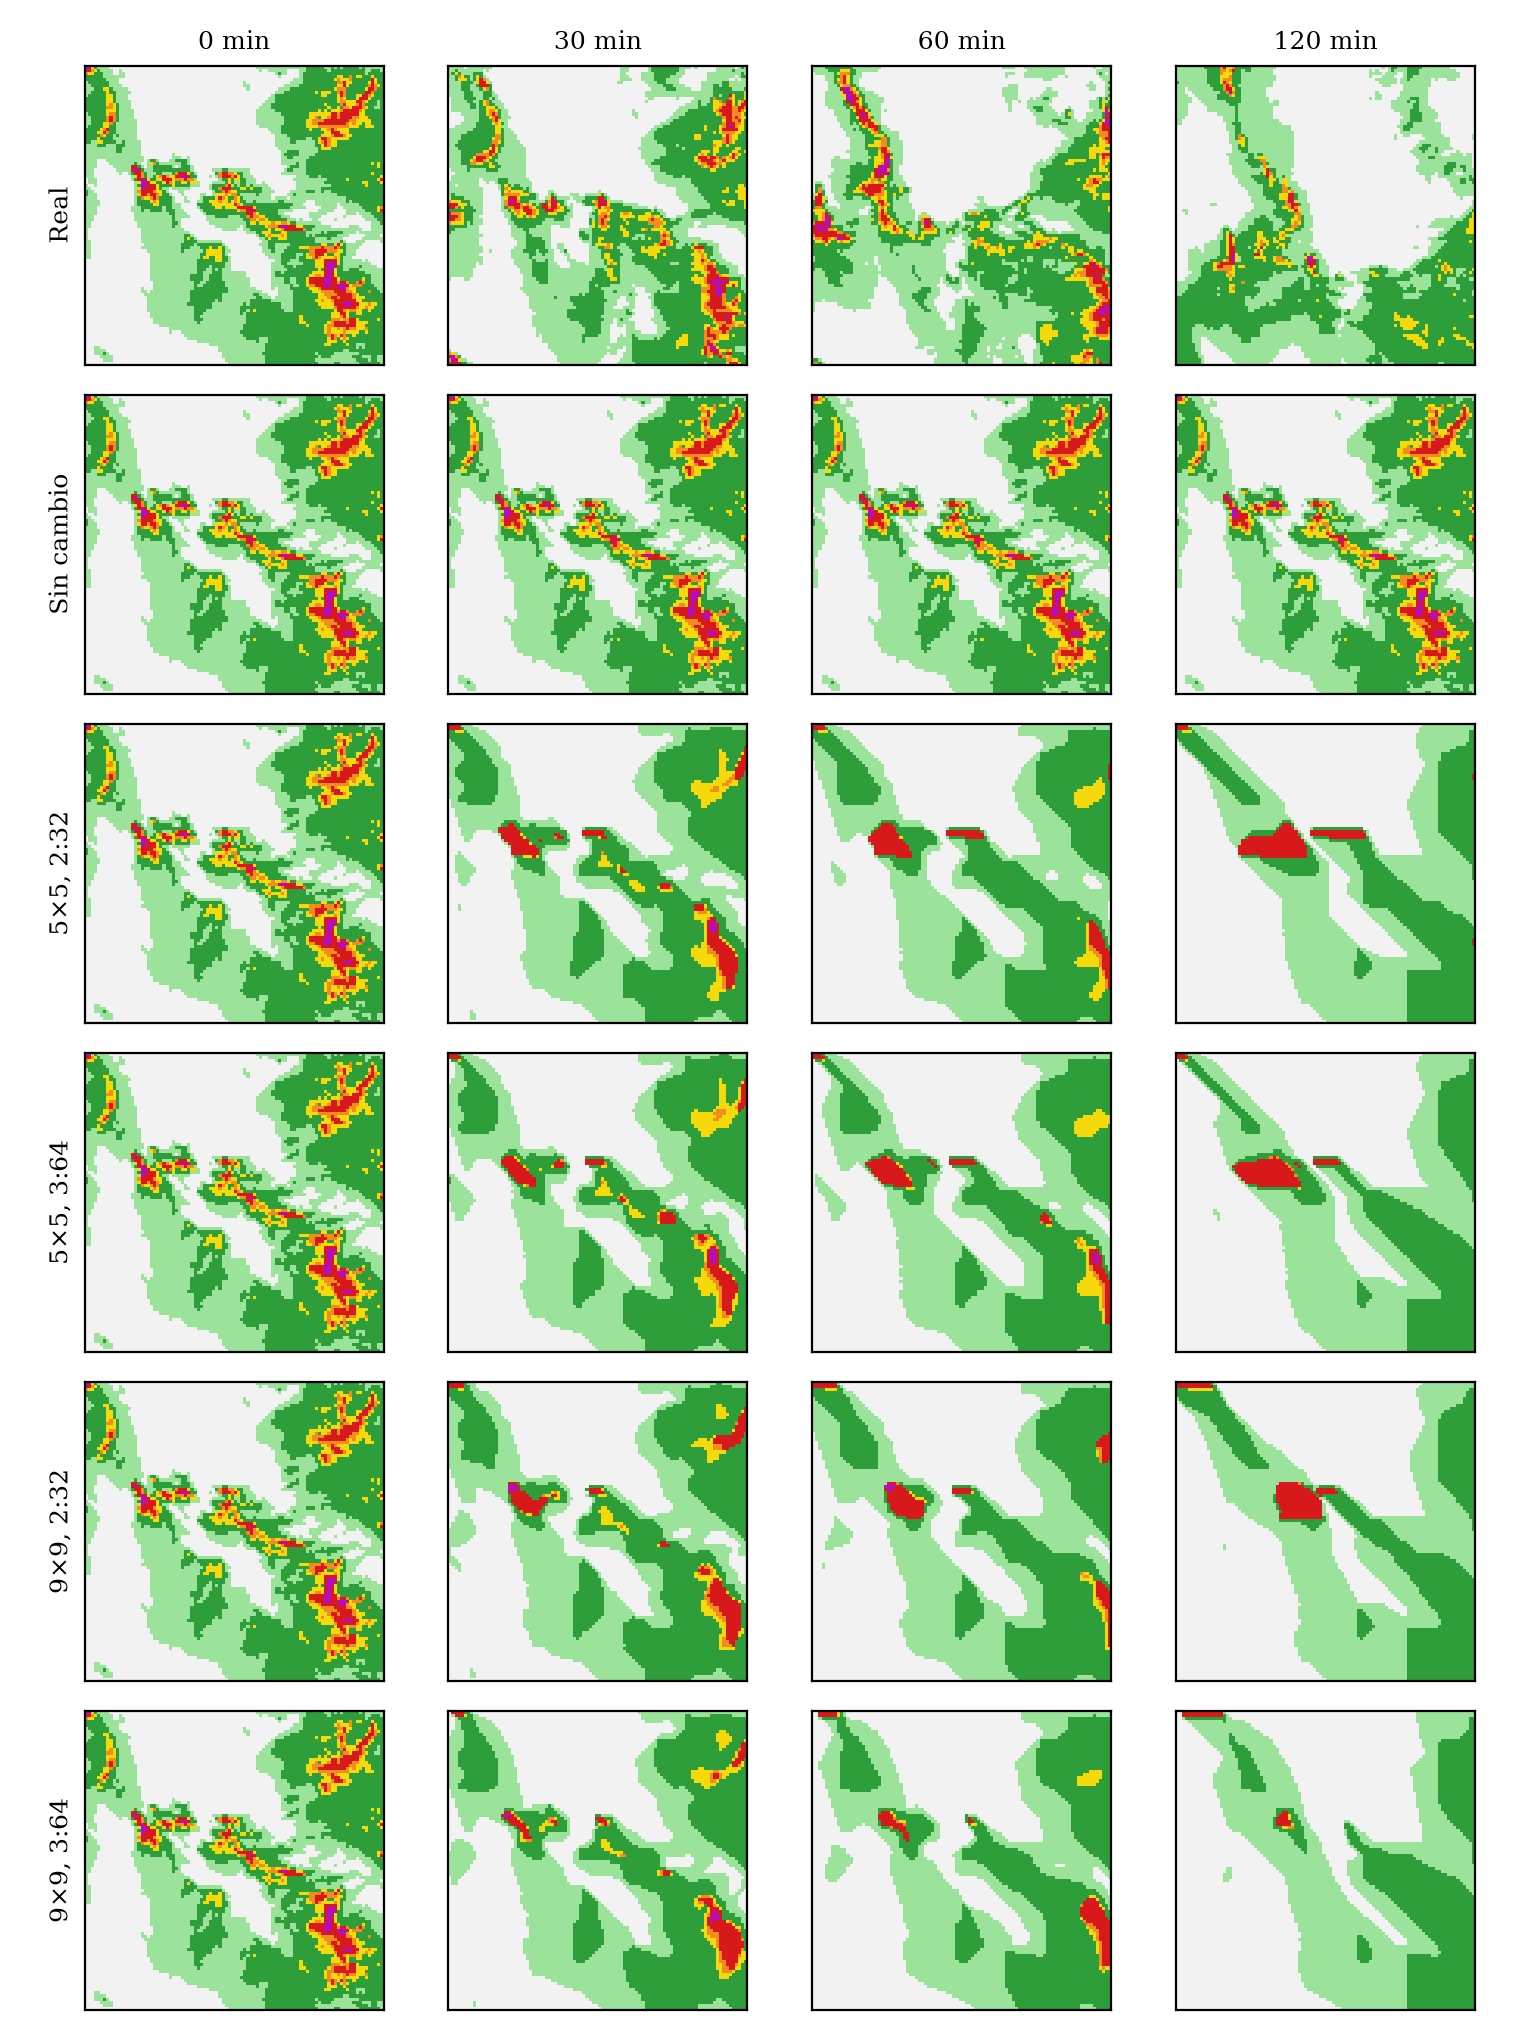
\includegraphics[width=0.78\linewidth]{sevir/comparacion.png}
	\leyendasevir
	\caption{Evolución real de una tormenta de prueba, predicción sin cambio y simulación libre de las 4 configuraciones iniciales a los 0, 30, 60 y 120 minutos.}
	\label{fig:sevir_comp}
\end{figure}

\subsubsection{Barrido de configuraciones}
Para descartar que el límite se debiera a la configuración, se entrenaron 80 redes que combinan 8 vecindades (de 25 a 121 vecinos), 5 tamaños de red (de 2:32 a 16:128) y entrada lineal o \onehot{}, probadas en 200 tormentas de 2019 (tabla~\ref{tab:sevir}). Todas superan a la predicción sin cambio, pero quedan muy cerca unas de otras: a los 60 minutos, el área con tormenta de la simulación libre va de 39.6 a 41.6\,\%. Las vecindades que llegan a 4 o más células de distancia son ligeramente mejores, pasar de 2:32 a 16:128 solo sube esa área de 40.3 a 40.8\,\% y ambas codificaciones dan prácticamente el mismo resultado. Entrenar con 400 tormentas de 5 transiciones mejora a 40 tormentas completas con casi el mismo número de transiciones, es decir, ayuda más la variedad que la cantidad, y las semillas aleatorias cambian el resultado hasta en 0.8\,\%, más que la diferencia entre muchas configuraciones.

\begin{table}[!t]
	\centering
	\footnotesize
	\setlength{\tabcolsep}{3pt}
	\caption{Exactitud y área con tormenta en 200 tormentas de prueba de 2019. Las vecindades muestran el promedio de 10 redes entrenadas con 40 tormentas.}
	\label{tab:sevir}
	\begin{tabular}{@{}lrrrr@{}}
		\toprule
		& & \multicolumn{3}{c}{\textbf{Área con tormenta}} \\
		\cmidrule(l){3-5}
		\textbf{Configuración} & \textbf{Exactitud} & \textbf{1 paso} & \textbf{60 min} & \textbf{120 min} \\
		\midrule
		Predicción sin cambio & 87.79\,\% & 77.98\,\% & 31.78\,\% & 20.02\,\% \\
		$5\times5$ (25 vecinos) & 90.13\,\% & 82.20\,\% & 40.02\,\% & 26.79\,\% \\
		Circular, radio 5 (81) & 90.17\,\% & 82.26\,\% & 40.89\,\% & 28.27\,\% \\
		Dispersa FLAME~3 (41) & 90.17\,\% & 82.28\,\% & 40.85\,\% & 28.00\,\% \\
		$11\times11$ (121) & 90.16\,\% & 82.26\,\% & 40.94\,\% & 28.33\,\% \\
		\midrule
		$11\times11$, 16:64, 400 tormentas & \textbf{90.34\,\%} & \textbf{82.67\,\%} & \textbf{41.83\,\%} & \textbf{28.84\,\%} \\
		\quad semilla 1 & 90.35\,\% & 82.63\,\% & 41.19\,\% & 27.56\,\% \\
		\quad semilla 2 & 90.33\,\% & 82.63\,\% & 41.02\,\% & 27.41\,\% \\
		\bottomrule
	\end{tabular}
\end{table}

Para saber qué aprendió la mejor red se midió el desplazamiento de cada tormenta en 60 minutos. Las tormentas reales se desplazan en promedio 5.82 células (23 km) hacia el este, con una desviación estándar de 7.06 células en la dirección este--oeste y 7.18 en la norte--sur; la red las desplaza 7.17 células (29 km) hacia el este con mucha menos variación (4.49 y 4.04), y su correlación con el desplazamiento real es débil (0.36 y 0.51). La red aprendió principalmente a mover las tormentas hacia el este, la dirección más común en Estados Unidos. La dirección y el crecimiento de una tormenta dependen del viento, la humedad y la temperatura a distintas alturas, que no están en las imágenes, y otras tormentas entran desde fuera del espacio: dos vecindades idénticas pueden tener futuros distintos, por lo que ninguna vecindad determina la transición. El límite no depende de los datos, de la red ni de la vecindad, sino de que las tormentas son un sistema abierto.

\subsection{Crecimiento de \textit{Physarum polycephalum}}

\textit{Physarum polycephalum} es un moho mucilaginoso capaz de resolver laberintos sin sistema nervioso. Se usó el conjunto de Harrington y Harrington \cite{harrington2026physarum}, con fotografías de 24 cajas de Petri de 90 mm con hojuelas de avena, en 4 experimentos de 6 cajas: 001 y 002, fotografiados cada 5 minutos durante 63 horas, y 008 y 009, cada 2 minutos durante 141 horas. A diferencia de las tormentas, la caja es un sistema cerrado: nada entra desde fuera y la condición inicial es la posición del moho y de la avena.

Las imágenes se recortaron al 90\,\% interior de la caja para evitar reflejos, cada una se sustituyó por la mediana de las de $\pm5$ minutos con la iluminación corregida y cada píxel se asignó a uno de 6 estados visibles: borde, fondo, avena y plasmodio tenue, medio e intenso. Después se redujeron de $320\times320$ a $160\times160$ células con el estado más común de cada bloque de $2\times2$, y un cambio de estado solo se aceptó si duraba al menos dos imágenes, ya que sin este filtro el 28\,\% de los cambios se revertía (figura~\ref{fig:physarum_pre}). La caja 5 de cada experimento se reservó para la prueba.

\begin{figure}[!t]
	\centering
	\begin{subfigure}[b]{0.24\linewidth}
		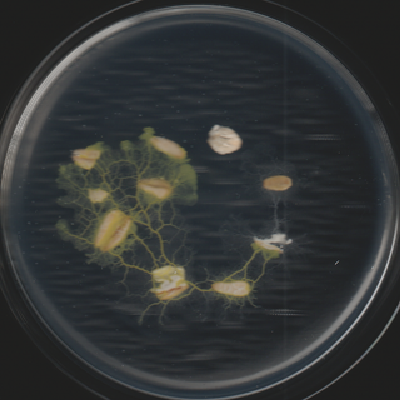
\includegraphics[width=\linewidth]{physarum/preprocesamiento_1.png}
		\caption{Original}
	\end{subfigure}\hfill
	\begin{subfigure}[b]{0.24\linewidth}
		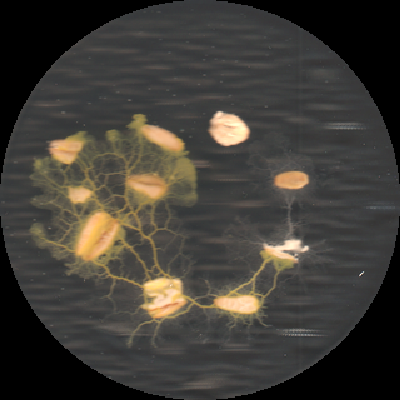
\includegraphics[width=\linewidth]{physarum/preprocesamiento_2.png}
		\caption{Limpieza}
	\end{subfigure}\hfill
	\begin{subfigure}[b]{0.24\linewidth}
		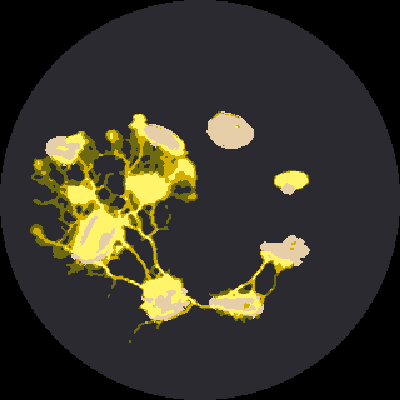
\includegraphics[width=\linewidth]{physarum/preprocesamiento_3.png}
		\caption{6 estados}
	\end{subfigure}\hfill
	\begin{subfigure}[b]{0.24\linewidth}
		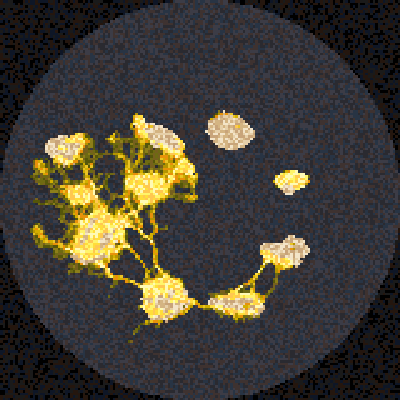
\includegraphics[width=\linewidth]{physarum/preprocesamiento_4.png}
		\caption{24 estados}
	\end{subfigure}
	\caption{Preprocesamiento de la caja 5 del experimento 008 a las 50 horas.}
	\label{fig:physarum_pre}
\end{figure}

\subsubsection{Estado más probable y sesgo de crecimiento}
Con transiciones de 30 minutos, la red acierta el 97.99\,\% de las células en un paso, casi lo mismo que la predicción sin cambio. Aunque la caja es un sistema cerrado, el crecimiento no está determinado por la vecindad: las células que se vuelven plasmodio en los siguientes 30 minutos tienen una probabilidad de solo 9\,\%. Como la regla elige el estado más probable, ninguna célula cambia y la simulación libre se congela. Elegir el estado al azar con las probabilidades de la red, lo que rompe la definición determinista del autómata, tampoco funciona: el plasmodio brota en toda la caja, aunque en los datos reales el 97.4\,\% del plasmodio nuevo aparece a 6 células o menos del existente.

Para crecer sin muestreo se sumó una constante a las salidas de plasmodio (un sesgo de crecimiento) y se alargó el paso de tiempo, ya que en pasos largos el crecimiento es menos incierto. Se entrenaron 122 redes y se evaluaron con la coincidencia del plasmodio (ecuación~\ref{eq:coincidencia}), en la que la predicción sin cambio obtiene entre 0.04 y 0.06 y llenar la caja de plasmodio, 0.07. El paso de tiempo es lo más importante (tabla~\ref{tab:physarum_paso}): la coincidencia sube de 0.120 con pasos de 30 minutos a 0.223 con pasos de 6 horas. La vecindad y el tamaño de la red casi no cambian el resultado, mientras que quitar la avena lo reduce a 0.134, es decir, la avena guía al plasmodio. Sin embargo, la mejor red crece en manchas sólidas, sin movimiento interno ni venas.

\begin{table}[!t]
	\centering
	\footnotesize
	\setlength{\tabcolsep}{4pt}
	\caption{Coincidencia del plasmodio en la simulación libre de las 4 cajas de prueba según el paso de tiempo (4 estados, 53 vecinos, \red{16:64:ReLU}{4:Linear}, \onehot{}). Plasmodio: fracción de la caja con plasmodio al final.}
	\label{tab:physarum_paso}
	\begin{tabular}{@{}lrcccc@{}}
		\toprule
		& & & \multicolumn{2}{c}{\textbf{Coincidencia}} & \textbf{Plasmodio} \\
		\cmidrule(lr){4-5}
		\textbf{Paso} & \textbf{Pérdida} & \textbf{Sesgo} & \textbf{Sin sesgo} & \textbf{Con sesgo} & \textbf{red / real} \\
		\midrule
		30 min & 0.0420 & 2.125 & 0.058 & 0.120 & 0.58 / 0.34 \\
		1 h & 0.0752 & 1.625 & 0.057 & 0.140 & 0.58 / 0.34 \\
		2 h & 0.1230 & 1.5 & 0.054 & 0.167 & 0.61 / 0.34 \\
		3 h & 0.1564 & 1.5 & 0.051 & 0.174 & 0.67 / 0.35 \\
		4 h & 0.1841 & 1.375 & 0.047 & 0.210 & 0.52 / 0.33 \\
		6 h & 0.2222 & 1.25 & 0.043 & \textbf{0.223} & 0.38 / 0.35 \\
		8 h & 0.2546 & 1.25 & 0.029 & 0.185 & 0.39 / 0.34 \\
		\bottomrule
	\end{tabular}
\end{table}

\subsubsection{Simulación con ruido}
El brillo del plasmodio real cambia de forma aleatoria: cada 30 minutos alrededor del 5\,\% del plasmodio cambia de nivel, y conocer el nivel anterior no ayuda a predecirlo. Para reproducirlo sin cambiar la definición del autómata, cada célula lleva además un valor de ruido $r \in \{0,1,2,3\}$ como parte de su estado, $\sigma = 4v + r$, donde $v$ es el estado visible, por lo que el autómata tiene 24 estados. En cada paso:

\begin{enumerate}
	\item El ruido, escrito con dos bits $r = 2a + b$, evoluciona con una versión bidimensional de la regla 30:
	\begin{equation}
		a' = a_{\text{izq}} \oplus (a \lor a_{\text{der}}) \oplus b, \quad
		b' = b_{\text{arr}} \oplus (b \lor b_{\text{ab}}) \oplus a,
	\end{equation}
	donde $\oplus$ es el o exclusivo y los subíndices indican el vecino de la izquierda, derecha, arriba y abajo. Aunque es determinista, los 4 valores aparecen con la misma frecuencia, no se parecen a los de los vecinos ni a los del paso anterior y no se repiten en 400 pasos.
	\item Una red maestra (53 vecinos, \red{16:64:ReLU}{6:Linear}, paso de 30 minutos) da la probabilidad de cada estado visible. Las probabilidades se acomodan una tras otra entre 0 y 1, y cada célula calcula un número entre 0 y 1 con el ruido de sus $9\times9$ vecinos, con más peso en los más cercanos; el estado que toma es el del tramo donde cae ese número. Así, un estado con probabilidad de 15\,\% sale en el 15\,\% de los casos y, como las células vecinas tienen números parecidos, cambian juntas, en manchas (figura~\ref{fig:physarum_ruido}).
	\item El plasmodio solo puede aparecer en una célula si ya hay plasmodio en su vecindad.
\end{enumerate}

\begin{figure}[!t]
	\centering
	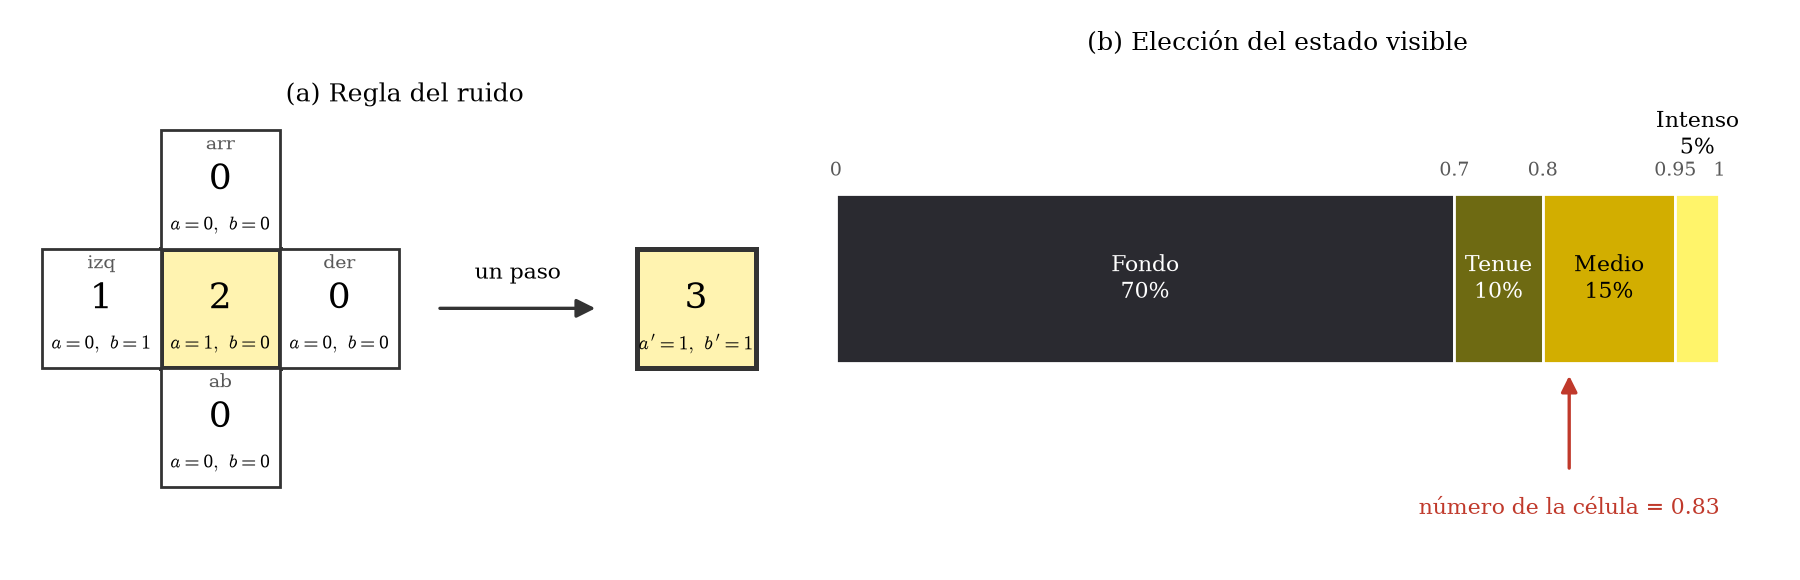
\includegraphics[width=\linewidth]{physarum/ruido_regla.png}
	\caption{Ejemplo de un paso con ruido. (a) La célula central tiene ruido 2 y pasa a 3 con la regla del ruido. (b) La red da la probabilidad de cada estado visible y el número de la célula (0.83) elige plasmodio medio.}
	\label{fig:physarum_ruido}
\end{figure}

Un segundo autómata celular neuronal aprende este procedimiento completo con 97 vecinos y la red \red{16:128:ReLU}{24:Linear} con \onehot{}, entrenada durante 30 épocas con 20 pares de imágenes reales y 20 simulados por caja. Como el objetivo de cada par es el resultado del procedimiento y no la imagen real siguiente, con el ruido como parte del estado la vecindad vuelve a determinar la transición y la red solo tiene que aprender una regla determinista: en un paso acierta el estado visible del 99.17\,\% de las células y el ruido del 99.98\,\%.

\begin{figure*}[!t]
	\centering
	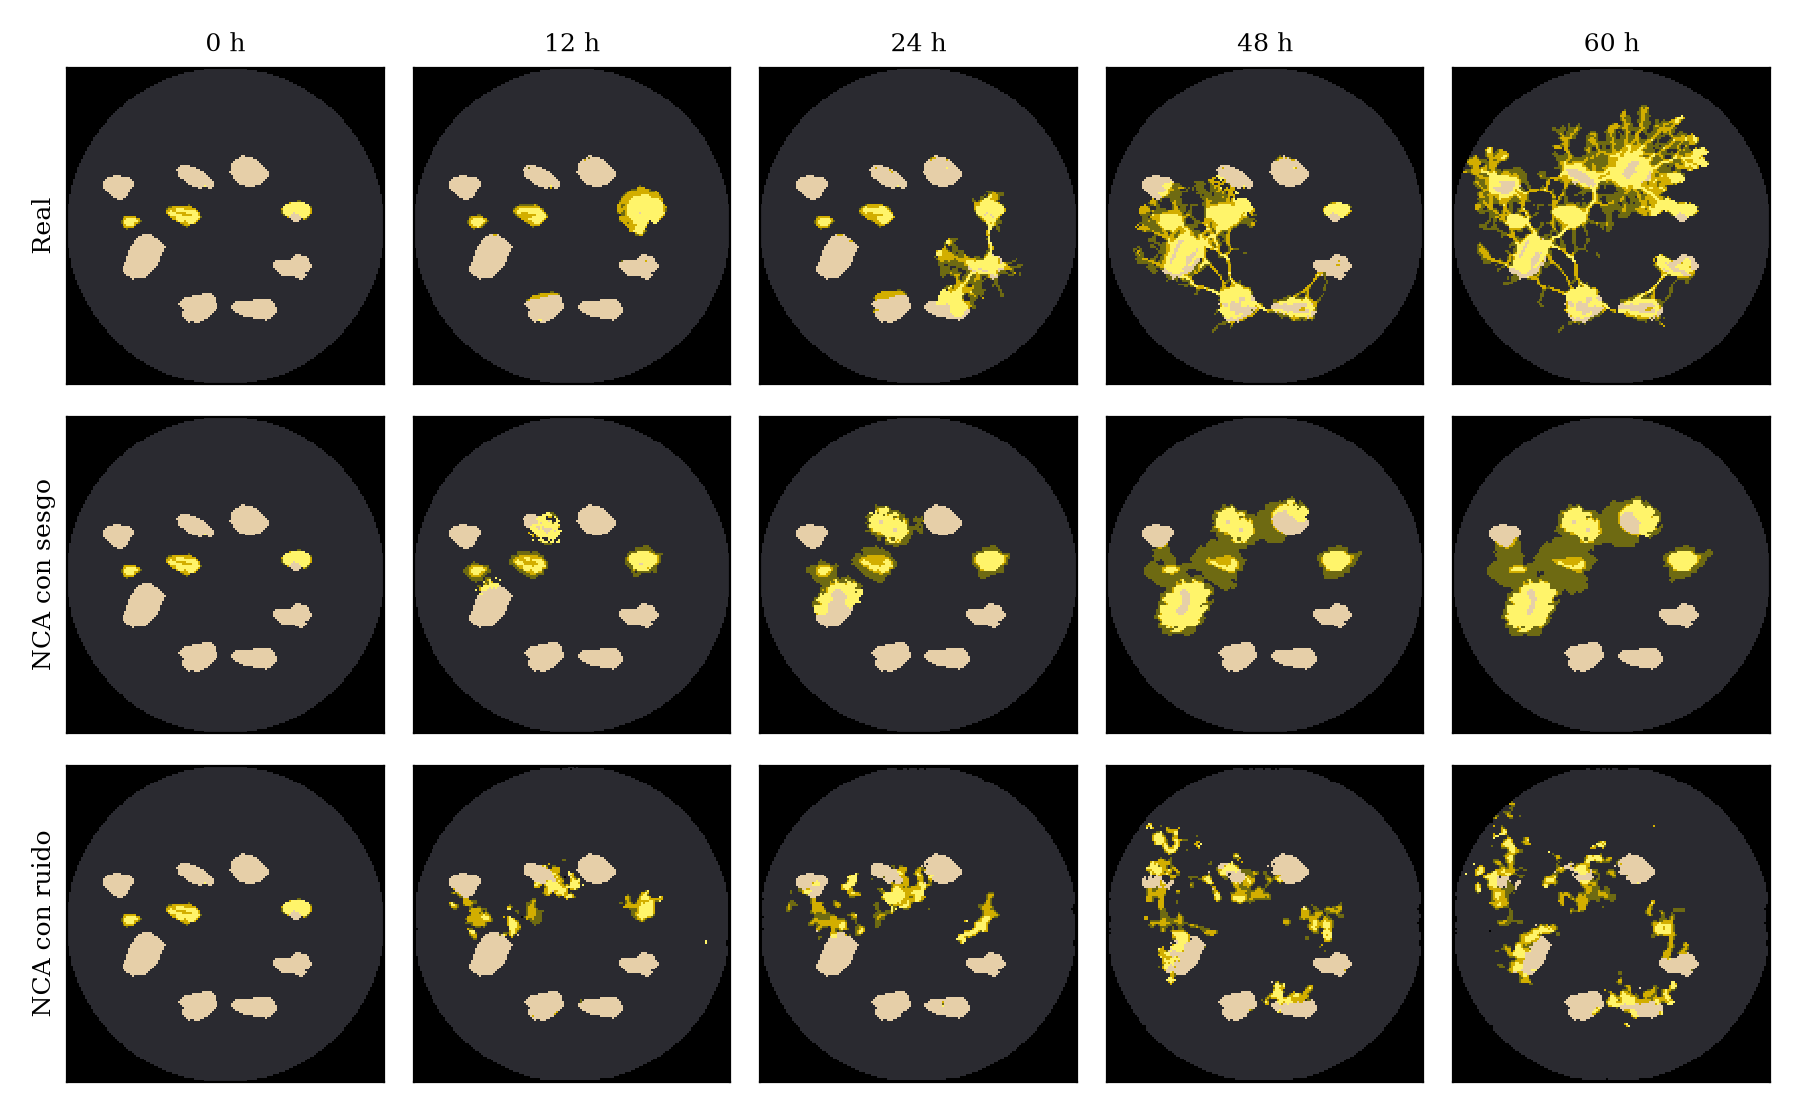
\includegraphics[width=0.72\textwidth]{physarum/comparacion.png}
	\caption{Evolución real de la caja 5 del experimento 008 y simulación libre del autómata celular neuronal con sesgo de crecimiento (6 estados, paso de 6 horas) y con ruido (24 estados, paso de 30 minutos), con los colores del estado visible.}
	\label{fig:physarum_comp}
\end{figure*}

\begin{table}[!t]
	\centering
	\footnotesize
	\setlength{\tabcolsep}{3pt}
	\caption{Simulación libre en las 4 cajas de prueba. Borde: fracción del plasmodio que toca una célula sin plasmodio (alta en ramas, baja en manchas). Cambio de brillo: fracción del plasmodio que cambia de nivel entre pasos.}
	\label{tab:physarum_comp}
	\begin{tabular}{@{}lccccc@{}}
		\toprule
		& & & & \multicolumn{2}{c}{\textbf{Cambio de brillo}} \\
		\cmidrule(l){5-6}
		& \textbf{Coincid.} & \textbf{Plasmodio} & \textbf{Borde} & \textbf{6 h} & \textbf{30 min} \\
		\midrule
		Real & -- & 0.344 & 0.429 & 23.6\,\% & 4.7\,\% \\
		Red con sesgo & \textbf{0.225} & \textbf{0.353} & 0.154 & 0.8\,\% & -- \\
		Red con ruido & 0.105 & 0.157 & \textbf{0.498} & 41.3\,\% & \textbf{6.5\,\%} \\
		\bottomrule
	\end{tabular}
\end{table}

La red con ruido reproduce la forma y el movimiento que le faltan a la red con sesgo (figura~\ref{fig:physarum_comp} y tabla~\ref{tab:physarum_comp}): el borde del plasmodio pasa de 0.154 a 0.498 (0.429 en la realidad), es decir, forma ramas en lugar de manchas, y el 6.5\,\% del plasmodio cambia de nivel cada 30 minutos, contra el 4.7\,\% real. El plasmodio crece desde el inóculo, avanza entre la avena y no aparece en zonas vacías. En cambio, crece menos que el real (15.7 contra 34.4\,\% de la caja) y su coincidencia es menor, algo esperado, ya que con ruido la red no puede saber hacia dónde crecerá cada rama, mientras que la red con sesgo crece en todas direcciones a la vez. Otras 20 redes con más épocas, otra reducción de la tasa de aprendizaje o un empujón de crecimiento suben la coincidencia de 0.115 a 0.136, pero solo porque crecen más, hasta cubrir cajas en las que el plasmodio real se queda alrededor de la avena. Ninguna red forma las venas largas que unen la avena ni sabe cuándo dejar de crecer. En los datos reales, el plasmodio que acaba de llegar a una célula se retira entre 4 y 6 veces más que el que lleva varias horas, por lo que las venas probablemente dependen de lo ocurrido durante horas, mientras que la red solo conoce el estado actual.

\subsection{Análisis comparativo}

La tabla~\ref{tab:sintesis} resume los seis experimentos, cuyos resultados se explican con las dos condiciones de la sección~\ref{sec:formulacion}. Cuando la vecindad determina la transición, como en los tres sistemas con regla conocida y en \textit{Physarum polycephalum} con el ruido como parte del estado, el autómata celular neuronal reproduce la evolución de entrenamiento. Cuando falta un vecino relevante o la evolución depende de variables que no están en el espacio, como en FLAME~3 y SEVIR, la mejor regla determinista elige el estado más probable y la dinámica se congela o se debilita. La cobertura explica los errores restantes: ante patrones ausentes en los datos, como las generadoras contiguas o la hormiga que se divide, la regla aprendida difiere de la original.

\begin{table}[!t]
	\centering
	\footnotesize
	\setlength{\tabcolsep}{3pt}
	\caption{Síntesis de los experimentos.}
	\label{tab:sintesis}
	\begin{tabularx}{\linewidth}{@{}lcX@{}}
		\toprule
		\textbf{Sistema} & \textbf{Cerrado} & \textbf{Resultado y limitación principal} \\
		\midrule
		Juego de la vida & Sí & Regla exacta con 1:4; sin un vecino relevante no se aprende. \\
		Pila de arena & Sí & 100\,\% de exactitud; generaliza parcialmente a generadoras contiguas. \\
		Hormiga de Langton & Sí & Sin errores en 8 de 9 reglas de hasta 50 estados; aplica la regla de colisión fuera de contexto. \\
		FLAME~3 & Parcial & Propaga el frente (área quemada de hasta 86\,\%), pero no las temperaturas; solo dos grabaciones. \\
		SEVIR & No & Mejor que sin cambio, pero solo desplaza las tormentas hacia el este. \\
		\textit{Physarum} & Sí & Ramas y movimiento interno con ruido; sin venas ni fin del crecimiento. \\
		\bottomrule
	\end{tabularx}
\end{table}

	\section{CONCLUSIONES}
\label{sec:conclusiones}

En este trabajo se planteó la simulación de sistemas complejos como un problema inverso: inferir, a partir de la evolución observada, la regla local de un autómata celular bidimensional, discreto, determinista y síncrono, definida por un perceptrón multicapa entrenado con las transiciones de cada célula. Se mostró que una regla así existe solo si la vecindad determina el siguiente estado, y seis experimentos permitieron responder a las preguntas de investigación.

\textbf{P1. Inferencia de reglas conocidas.} El autómata celular neuronal infiere las reglas de los tres sistemas conocidos: el juego de la vida con una sola capa oculta de 4 neuronas, la pila de arena con el 100\,\% de exactitud y la hormiga de Langton con hasta 50 estados, aunque en cada paso solo cambian dos células. Sin embargo, reproducir la evolución de entrenamiento no garantiza haber extraído la función de transición completa: ante patrones ausentes en los datos, como dos generadoras contiguas o una hormiga que aplica fuera de contexto la regla de colisión, la red se equivoca, aunque su comportamiento sigue siendo similar al original.

\textbf{P2. Configuración de la red.} Basta una red pequeña, con ReLU en las capas ocultas, Linear en la salida y pocas capas con más neuronas. Con más de dos estados, la codificación \onehot{} es la mejora más importante, ya que evita relaciones lineales falsas entre estados y redujo 63 veces las épocas necesarias. La vecindad debe contener a todos los vecinos que influyen en la transición: sin uno solo de ellos la regla no puede aprenderse, mientras que una vecindad mayor no lo impide.

\textbf{P3. Parámetros de entrenamiento.} Cuando el entrenamiento es incompleto, la pérdida objetivo determina la regla aprendida. B3/S23 resultó estable, pues solo aprende la regla exacta o la regla en la que todo muere, mientras que las reglas que generan vida adicional derivan hacia otras reglas, no siempre semitotalísticas, porque la red casi nunca observa los patrones de baja frecuencia. La reducción de la tasa de aprendizaje por \textit{plateau} elimina las oscilaciones de la pérdida y permite alcanzar pérdidas objetivo exigentes.

\textbf{P4. Condiciones de un sistema real.} El sistema debe ser cerrado y su estado debe contener la información de la transición. En \textit{Physarum polycephalum}, un sistema cerrado, el autómata aprende el crecimiento del moho: el plasmodio crece desde el inóculo, la avena lo guía y no aparece en zonas vacías. El paso de tiempo fue el factor más importante para crecer con el estado más probable, y un valor de ruido incorporado al estado permitió reproducir la parte aleatoria del crecimiento con una regla determinista. En FLAME~3 la regla aprendida propaga el frente hacia las zonas correctas, extingue los frentes al colisionar y no vuelve a encender el terreno quemado, pero las temperaturas, la velocidad y la dirección dependen de dos grabaciones y de variables no registradas, como el relieve o el viento. En SEVIR la red supera a la predicción sin cambio en tormentas que nunca vio, pero solo aprende a desplazarlas hacia el este, un límite que no depende de los datos, de la red ni de la vecindad, sino de factores externos al espacio.

En conclusión, la hipótesis se cumple en los sistemas cerrados, cuya evolución depende únicamente de los estados de las células: el juego de la vida, la pila de arena, la hormiga de Langton y el crecimiento de \textit{Physarum polycephalum}. Se cumple parcialmente en la propagación del fuego, limitada por las variables que no se registran y por la cantidad de datos, y no se cumple en sistemas abiertos como las tormentas.

\subsection{Trabajo a futuro}

A partir de las limitaciones observadas se proponen las siguientes líneas de investigación:

\begin{enumerate}
	\item \textbf{Memoria en el estado.} Incorporar al estado información de pasos anteriores, como se hizo con el ruido, para que la red pueda formar las venas de \textit{Physarum polycephalum}, cuyo plasmodio reciente se retira entre 4 y 6 veces más que el establecido.
	\item \textbf{Más datos de incendios.} Obtener grabaciones cenitales que registren el relieve, la vegetación y el viento, y representarlos como estados fijos del espacio para reducir la incertidumbre de la transición.
	\item \textbf{Autómatas celulares probabilísticos.} Estudiar reglas que elijan el siguiente estado con las probabilidades de la red, lo que cambia la definición de autómata celular usada en este trabajo.
	\item \textbf{Búsqueda y comparación de reglas.} Desarrollar métodos para buscar reglas con un comportamiento de interés y medir la similitud entre dos reglas, ya que las de los autómatas celulares neuronales se obtienen mediante entrenamiento y no se diseñan a mano.
\end{enumerate}

	\section*{RECONOCIMIENTOS}

Los Autores agradecen a la Escuela Superior de Cómputo del Instituto Politécnico Nacional por el apoyo recibido y las facilidades otorgadas para el desarrollo del presente trabajo terminal.

	% Bibliografía en formato BibTeX
	\bibliographystyle{IEEEtran}
	{\footnotesize\bibliography{referencias}}

\end{document}
